\documentclass[12pt, a4paper]{article}

\usepackage[utf8]{inputenc}
\usepackage[english]{babel}

% images %
\usepackage{graphicx} % to embed images
\graphicspath{ {IMG/} } % images are all in the same folder
\usepackage{subcaption} % for creating composite images
\usepackage[export]{adjustbox}
\usepackage{float}
% -- %

\usepackage{hyperref} % to link the table of contents
\usepackage{placeins} %floating
\usepackage{pdflscape} % to allow single pages in landscape mode
\usepackage[top=1.2in, bottom=1.2in, left=1in, right=1in]{geometry}

% include hyperlinks %
\usepackage{hyperref}
\hypersetup{
    colorlinks=true,
    linkcolor=black,
    urlcolor=blue,
}
% -- %

% algorithms %
\usepackage[ruled, vlined, linesnumbered]{algorithm2e} % algorithms
\usepackage{eurosym}
\usepackage{amssymb}
% -- %

\title{Design Document}
\date{2017-10-26}
\author{
	Leonardo Bisica
	\and
	Alessandro Castellani
	\and
	Michele Cataldo
}

\begin{document}
	%%% titlepage %%%
	\begin{titlepage}
		\centering
		
\includegraphics[width=5cm]{img/polimi_logo}
		\vfill
		{\bfseries\Large
			Travlendar+\\
			Design Document\\
			Version 1.0\\
			\vskip4cm
			Leonardo Bisica\\
			Alessandro Castellani\\
			Michele Cataldo\\
		}
		\vfill
		\vfill
	\end{titlepage}

%%% TABLE OF CONTENTS %%%
	\tableofcontents
	
	
	
%%% 1 - INTRODUCTION %%%
	\newpage
	\section{Introduction}
		\subsection{Purpose}
The purpose of this Design Document is to explain the architecture of the Travlendar+ mobile application as well as the logic underlying its development. Our approach will be analyzed in detail section by section, keeping, above all, coherence with the path our RASD layed down.

\subsection{Scope}
\textit{Travlendar+} is a mobile application that encompasses many different functionalities. 
It is first of all an event scheduler that keeps track of a user’s appointments so that it can display the fastest routes available, These routes are indexed by transportation means thanks to external APIs.
\textit{Travlendar+} heavily relies on "\textit{Google Maps APIs}" for tracking distances and travel times, but also uses the necessary APIs to locate and rent vehicles of sharing services and to buy public transportation tickets. Thanks to its ability to gather external info about weather, strikes and traffic, as well as average travel time, \textit{Travlendar+} can warn its users before creating an appointment (and during travel itself) if any overlap happens or if an event location can’t be reached in the expected time.

\subsection{Definitions, Acronyms, abbreviations}
We assume our Glossary already cover all the terms we introduced and specified in the RASD. In addition to that, we can add some additional word to our vocabulary :

Abbreviations :
\begin{description}
	\item[RASD] The Requirements Analysis and Specifications Document is the first document we produced in order to lay the foundations of Travlendar+.
	\item[DD] The Design Document is the document at hand.
	\item[API] Application Programming Interface.
	\item[Travel Logic] By travel logic we refer to the logic that processes the distances and the transportation time within our operative and influcence zones. In the case at hand, in this first implementation, we're going to adopt as Travel Logic the Google Maps APIs.
	\item[User]  The user is the final customer of \textit{Travlendar+}, the ones which uses the mobile application we detail.
	\item [RWn] The $n^{th}$ runtime view.
\end{description}

\subsection{Reference Documents}
\begin{itemize}
		\item[-] \textsf{Specification Document: Mandatory Project Assignments}, available in the BeeP page of the course.
\end{itemize} 

\subsection{Document Structure}
The document is organized into 7 sections:

\begin{itemize}
	\item Section 1 (Introduction): the section at hand. It provides the scope of our project and frames our DD.
	\item Section 2 (Architectural Design): this section details the architecture of \textit{Travlendar+}. It contains component, deployment and runtime views.
	\item Section 3 (Algorithm Design): this section displays the most important algorithms used by the mobile application.
	\item Section 4 (User Interface Design): this section briefly refers to the User Interface developed in the RASD.
	\item Section 5 (Requirements Traceability): this section tracks the requirements detailed in the RASD into their corresponding design elements.
	\item Section 6 (Implementation, Integration and Test Plan): this section identifies the order in which we implement the various subcomponents of the system as well as the order we want to implement and test them in.
	\item Section 7 (References and Used Tools): this section accounts for the references of our project, and the tools we adopted in order to write down and deliver this document.
\end{itemize}

		

%%% 2 - ARCHITECTURAL DESIGN  %%%
	\newpage
	\section{Architectural Design}
		\subsection{Overview}

	As we anticipated, in this section we’re goint to give an array of views of our system, shaping it from many angles at once. We’ll detail both the high-level components and the interfaces interleaved among them, delving then into deployment and runtime view.
	[Check] The architectural style we chose to adopt is a three-layered one.
	The decision to implement an external DB was born because of the need of providing a realiable and safe synchronization tool for our users and to store other kinds of personal information submitted through the app (like preferences and the like).
	Since the client implements travel logic and actually consists in the mobile application we’re aiming to develop, we are without any doubt in the frame of a fat client design.
	
\subsection{Component View}
	The Component Diagram shown below describes the logical components of the system we are to develop, from a very high-level description on to a more detailed one. This diagram does not take into account the deployment phase, hence it doesn’t describe the logical layer of the system in terms of the physical tiers where it is deployed.

\begin{figure}[H]
		\centering
		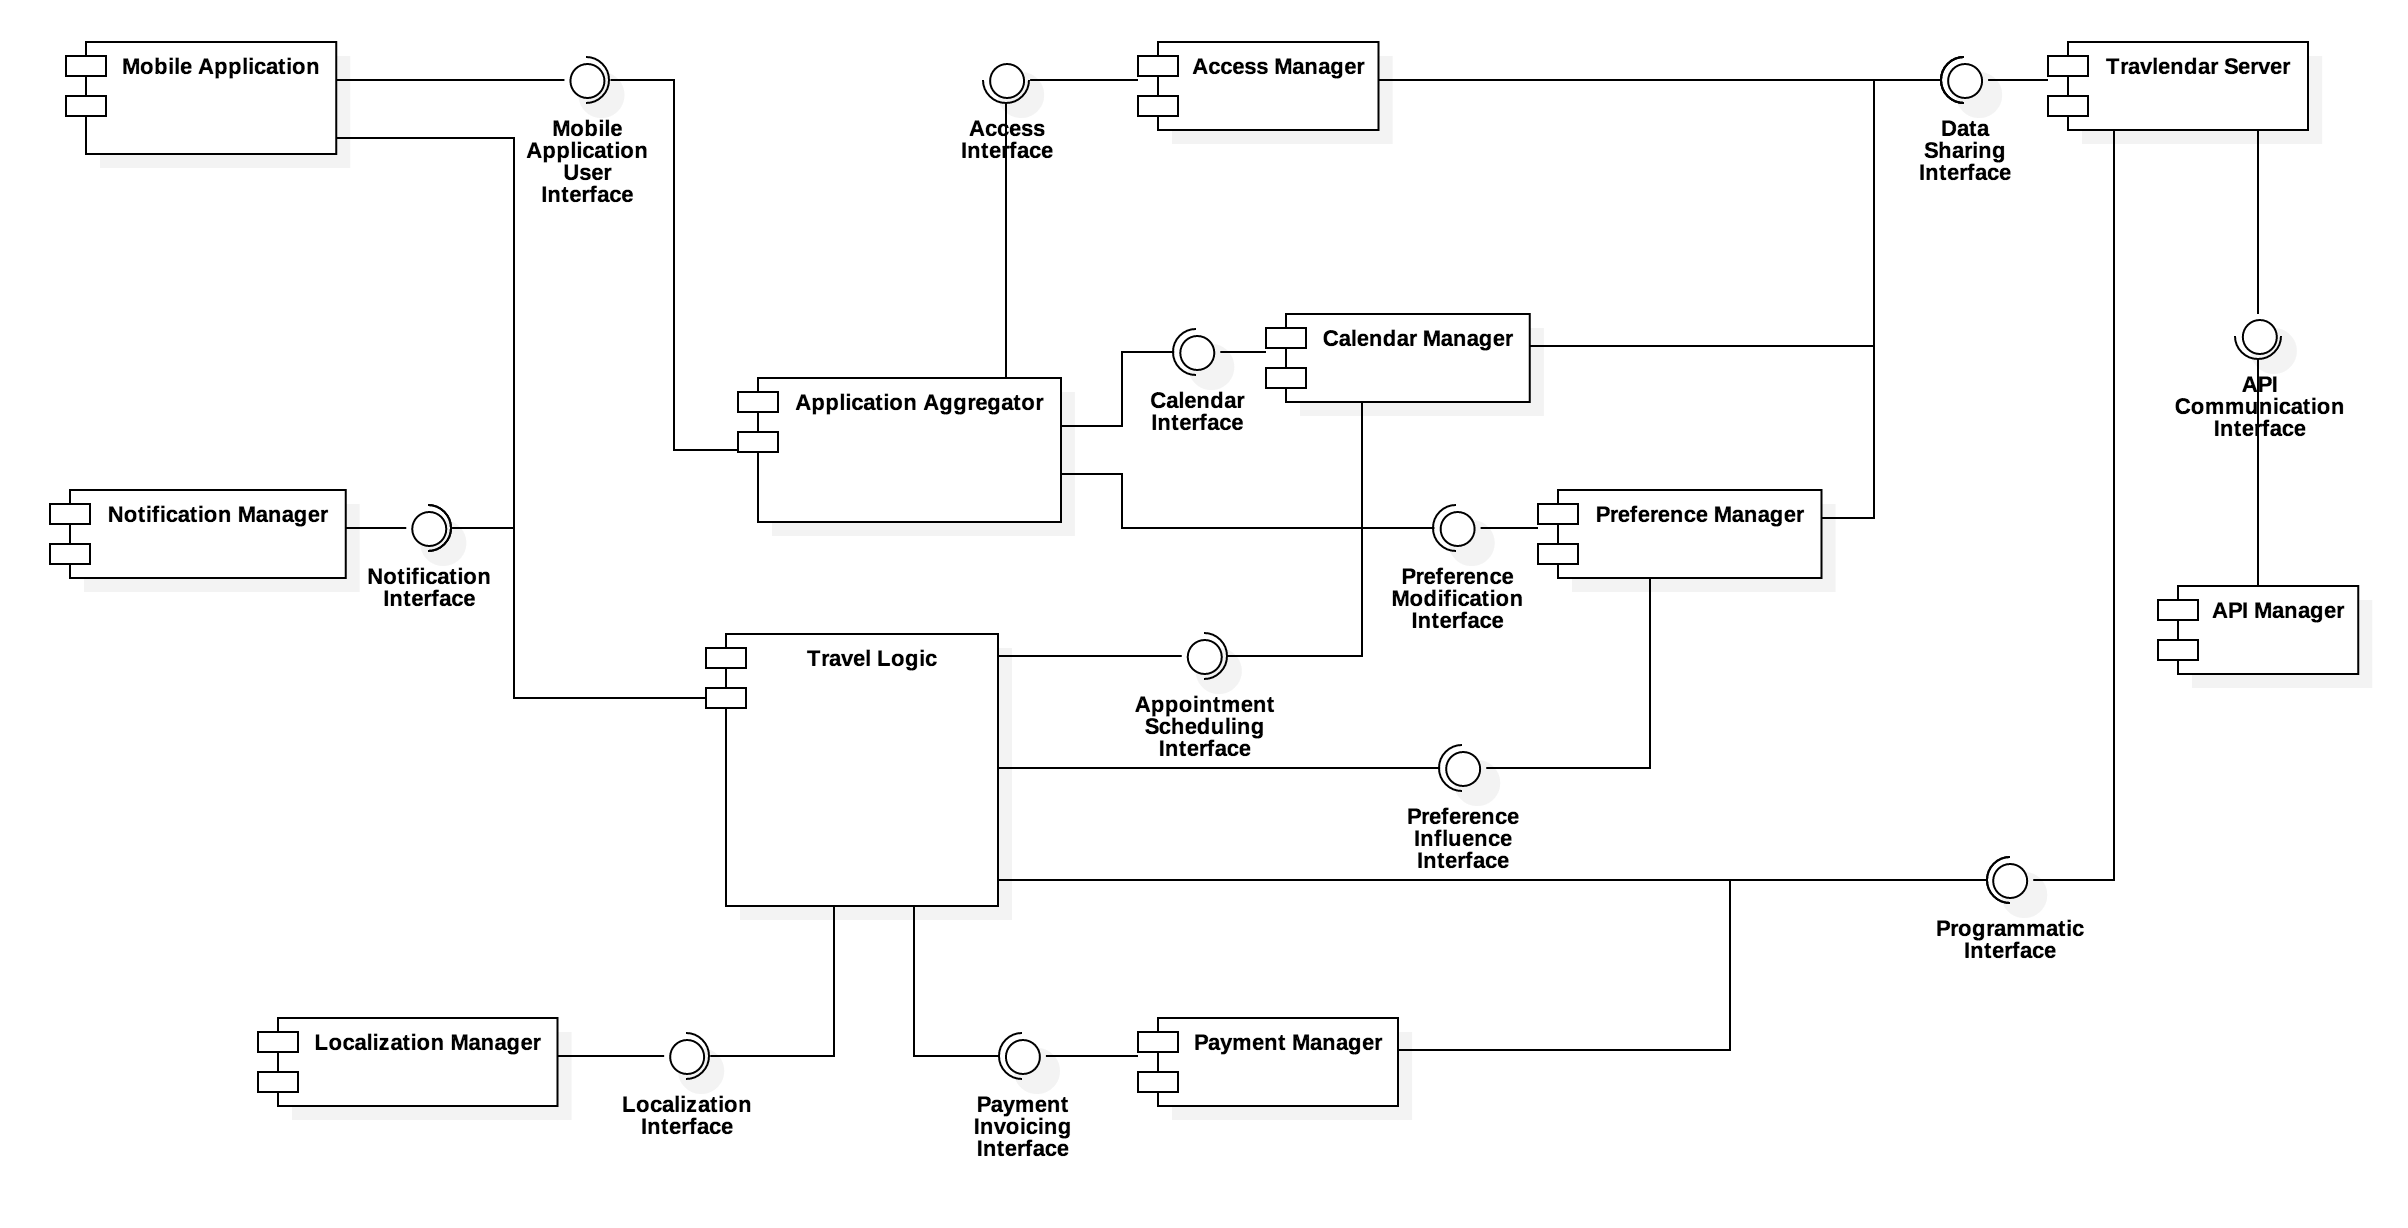
\includegraphics[width = \textwidth]{UML/componentDiagrams/highLevel}
		\caption{High level view}
		\label{componentHighLevel}
	\end{figure}

\paragraph{Mobile Application}
	This component represents the view of the User over its system. It’s split in two sub-components, Guest-view and User-view, which represents the two different ways an human interaction can be instaurated with the system.

	\begin{figure}[H]
		\centering
		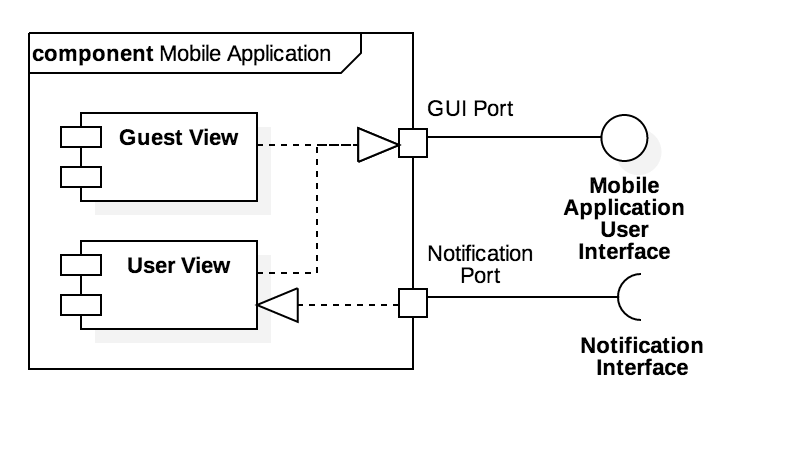
\includegraphics[scale = 0.2]{UML/componentDiagrams/mobileApplication}
	\end{figure}


\paragraph{Application Aggregator}
	This component works, unsuprisingly, as a collector of the different information \textit{Travlendar+} manages. It allows an easy management of every piece of information and allows us to avoid an high number of interfaces among the different components. 'Profile Manager' specifies the profile setting of the current user, while 'User Action Handler' allows us to register User's input.
	
	\begin{figure}[H]
		\centering
		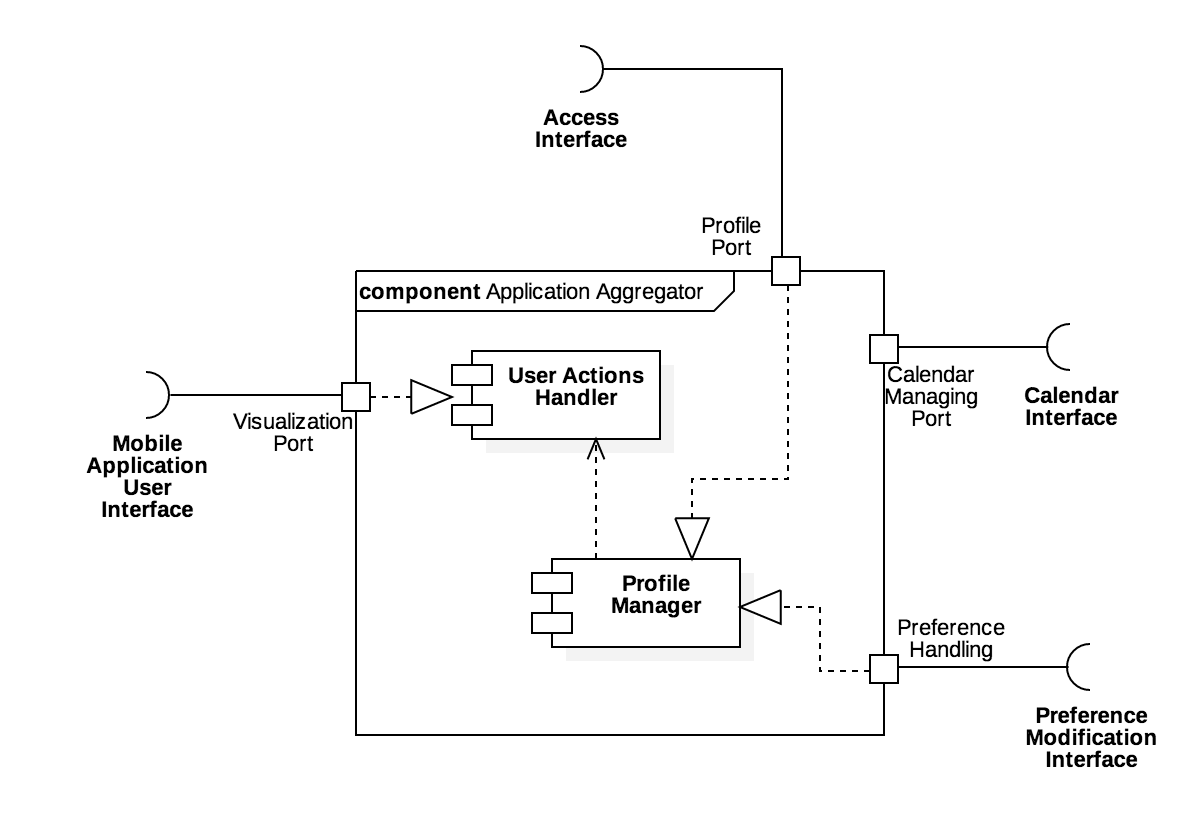
\includegraphics[scale = 0.2]{UML/componentDiagrams/applicationAggregator}
	\end{figure}
 
\paragraph{Calendar Manager}
	This component is divided into 'Appointments' and 'Breaks' sub-components, which track the appointments inserted by the User together with his breaks, and 'Trips', which is the list of trips arranged by the scheduler for every appointment. The sub-component 'Appointment Aggregator' serves the purpose of listing and presenting the content of the other two sub-components.
	
	\begin{figure}[H]
		\centering
		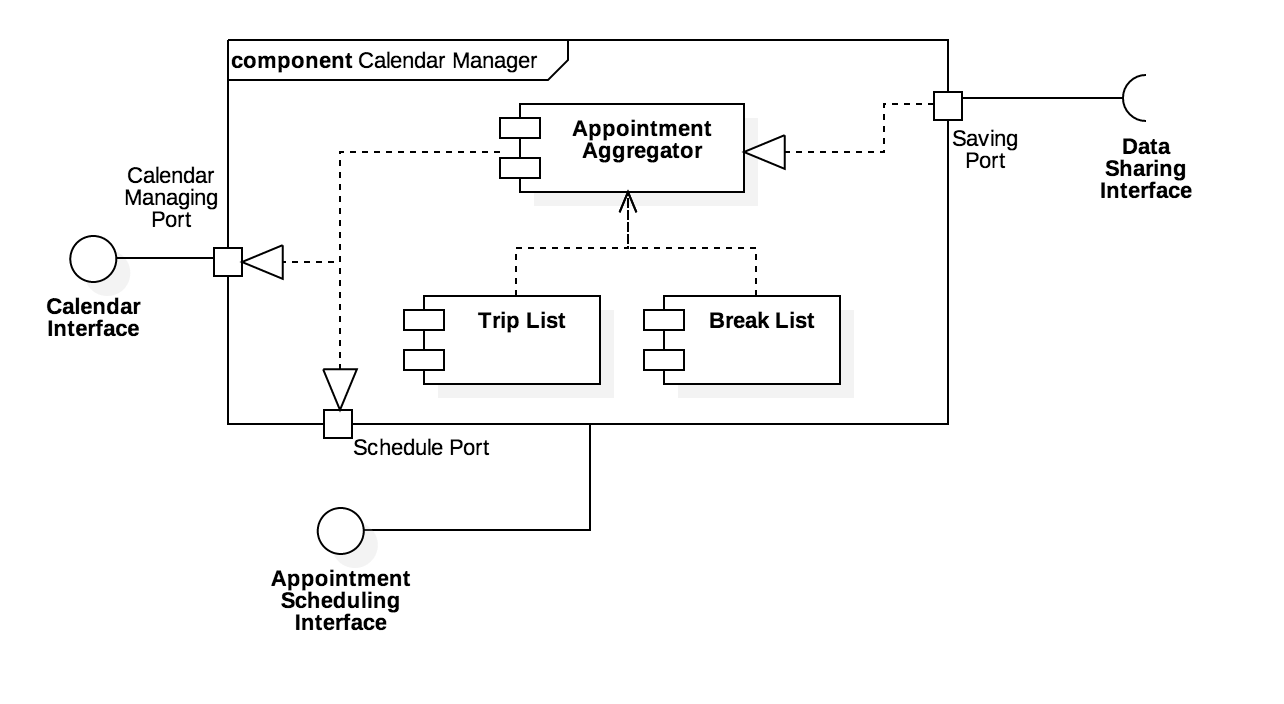
\includegraphics[scale = 0.2]{UML/componentDiagrams/calendarManager}
	\end{figure}
 

\paragraph{Preference Manager}
	This component serves the purpose of keeping track of the preferences expressed by the User. 'Season Pass Handler' takes care of storing season passes; 'Excluded Vehicles List' cuts off from the scheduler results involving a selection of banned transportation means, 'Preferences List' covers the remaining and wider spectrum of User's choices. 'Preference Handler' is the sub-component that manages the other ones and that communicates outside Preference Manager.

	\begin{figure}[H]
		\centering
		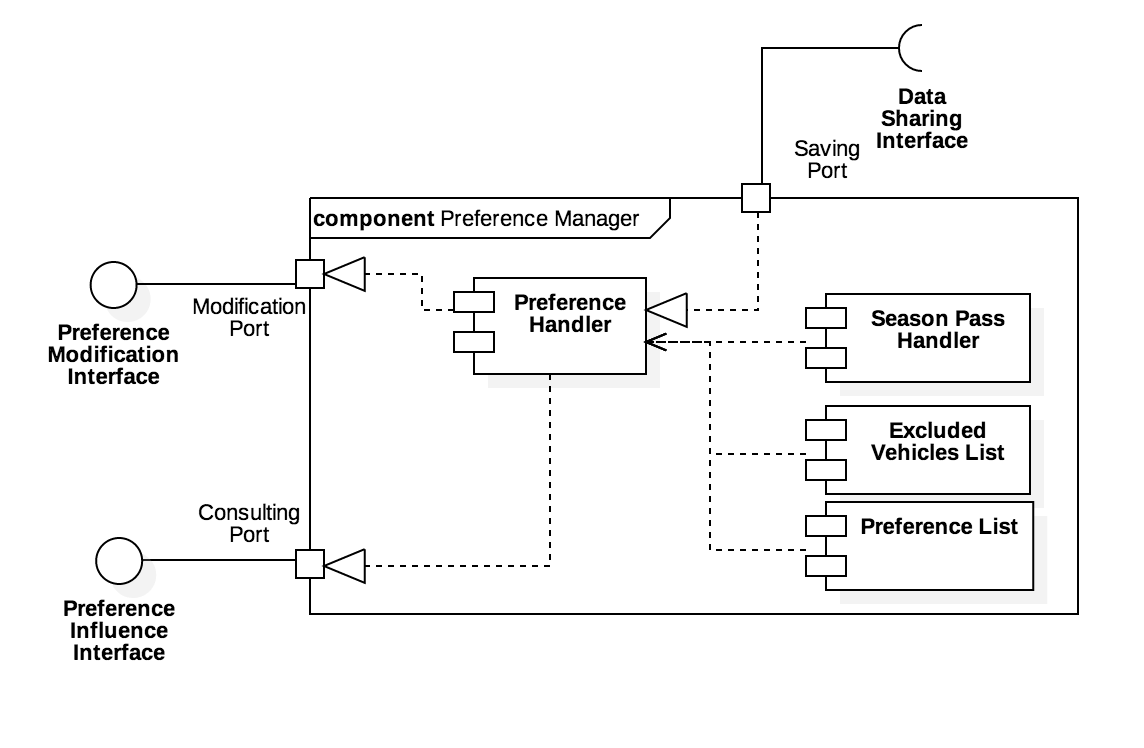
\includegraphics[scale = 0.2]{UML/componentDiagrams/preferenceManager}
	\end{figure}
	

\paragraph{Travlendar Server} 
	This component represents the \textit{Travlendar Server} whose purpose is to store User's preferences, access data and personal information. It is modeled by its 'DBMS' component, which stores Timetables and Preferences and the 'API Request Dispatcher', which forwards requests to external agents.

	\begin{figure}[H]
		\centering
		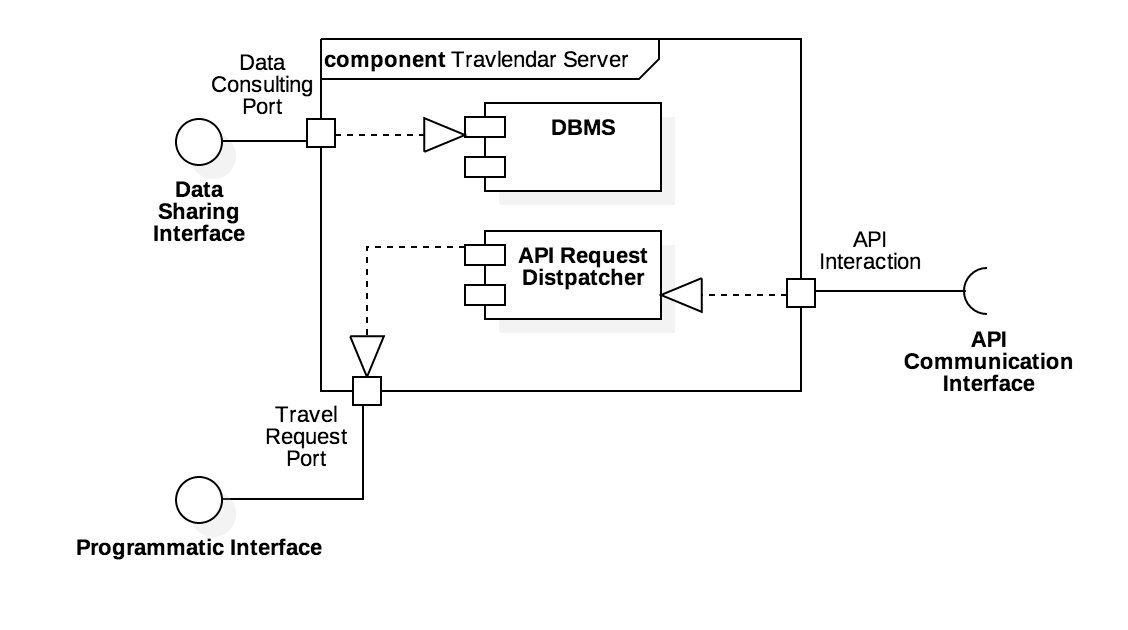
\includegraphics[scale = 0.2]{UML/componentDiagrams/travlendarServer}
	\end{figure}
	

\paragraph{Travel Logic Manager}
	This component is split into two sub-components: 'Scheduler' is the fundamental block that aims at scheduling and arranging User appointments and breaks via the the corresponding trips, 'DistanceManager' is the block whose purpose is to organize and present travel times to the scheduler in order to have them sorted out and well-managed.

	\begin{figure}[H]
		\centering
		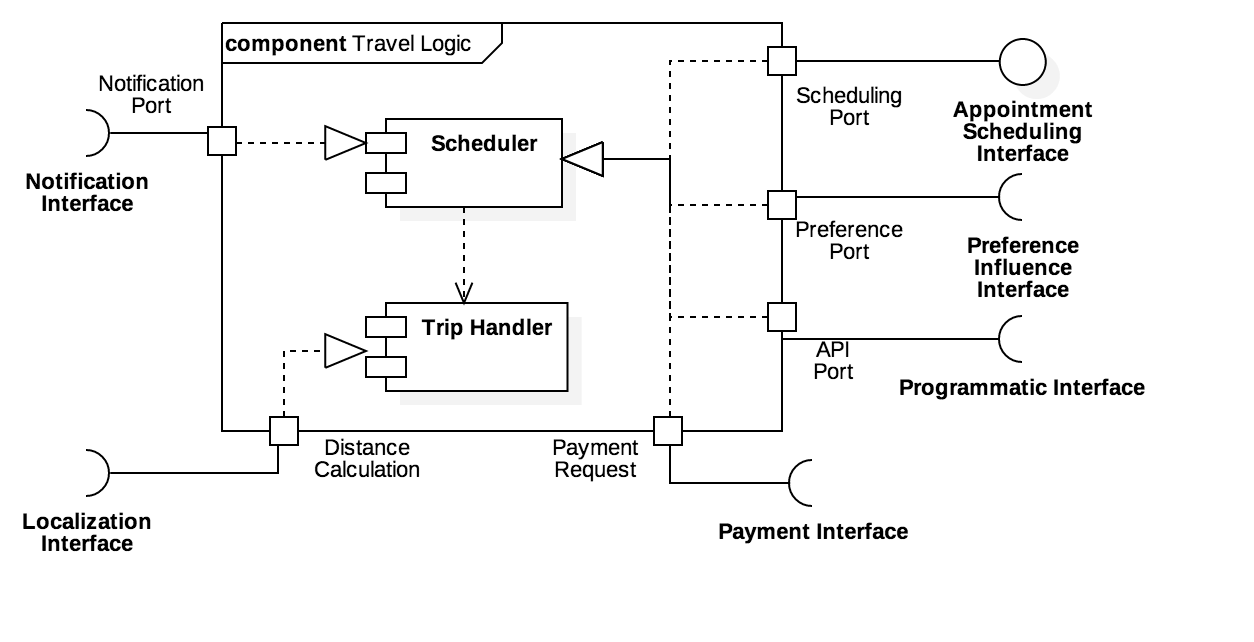
\includegraphics[scale = 0.2]{UML/componentDiagrams/travelLogic}
	\end{figure}
	

\paragraph{Payment Manager}
	This component deals with the recording of purchases and their associated credit cards.
	The sub-component 'Payment Handler' tracks purchase records and interacts with the required apps installed on the mobile device, while 'Purchase History' is an exploitable and rational organizations of the credit cards used by the user.

	\begin{figure}[H]
		\centering
		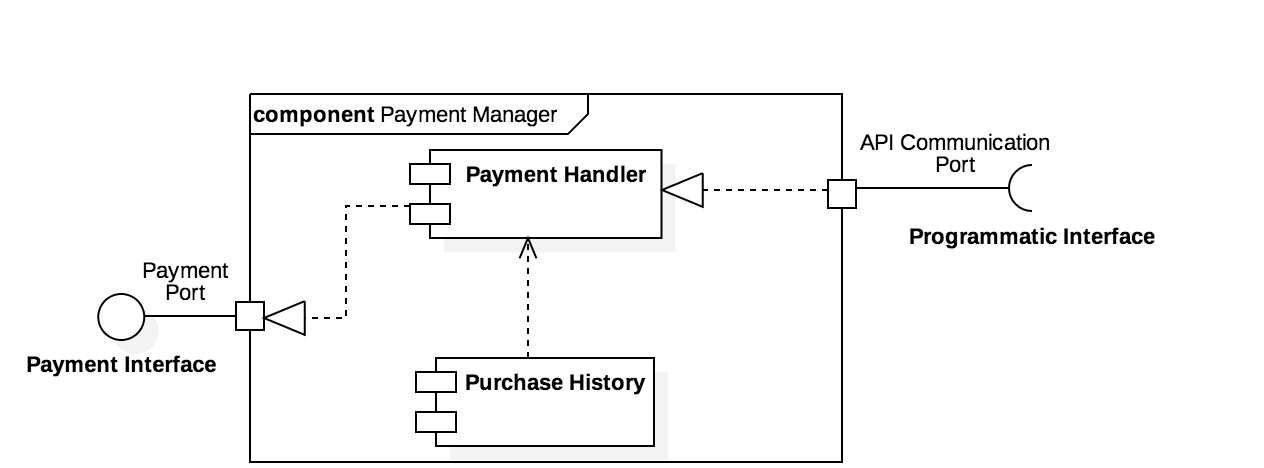
\includegraphics[scale = 0.2]{UML/componentDiagrams/paymentManager}
	\end{figure}
	

\paragraph{API Manager} 
	This component is critical in order to provide a functioning Travel Logic: it gathers the interactions with all external APIs.
	Here are listed the APIs the mobile application project starts with : Google Maps API, Google Transit API, Open Weather Map API, Car2Go and BikeMi API.
	The last couple is for reference only, as already pointed in the RASD. Naturally, the list of external services can be expanded.
	The 'Listener' component serves the purpose of forwarding requests and receives the desired inputs.
	
	\begin{figure}[H]
		\centering
		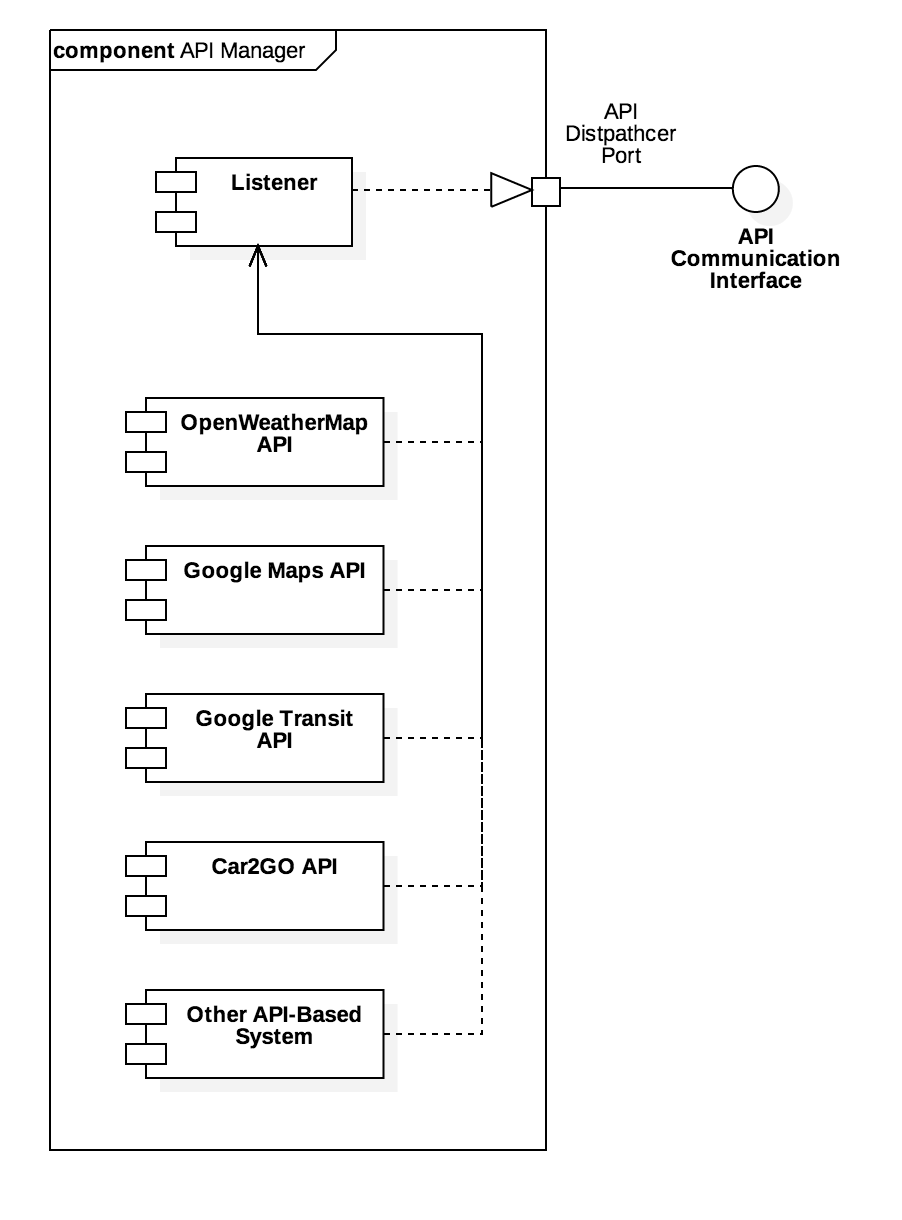
\includegraphics[scale = 0.2]{UML/componentDiagrams/APIManager}
	\end{figure}
	
	
\paragraph{Notification Manager}
	This component allows the notification system to warn users in the cases events partially or completely overlap according to the scheduler.

\paragraph{Localization Manager}
	This component represents the localization functionalities of the mobile application.
	
\begin{landscape}
	\begin{figure}
		\centering
		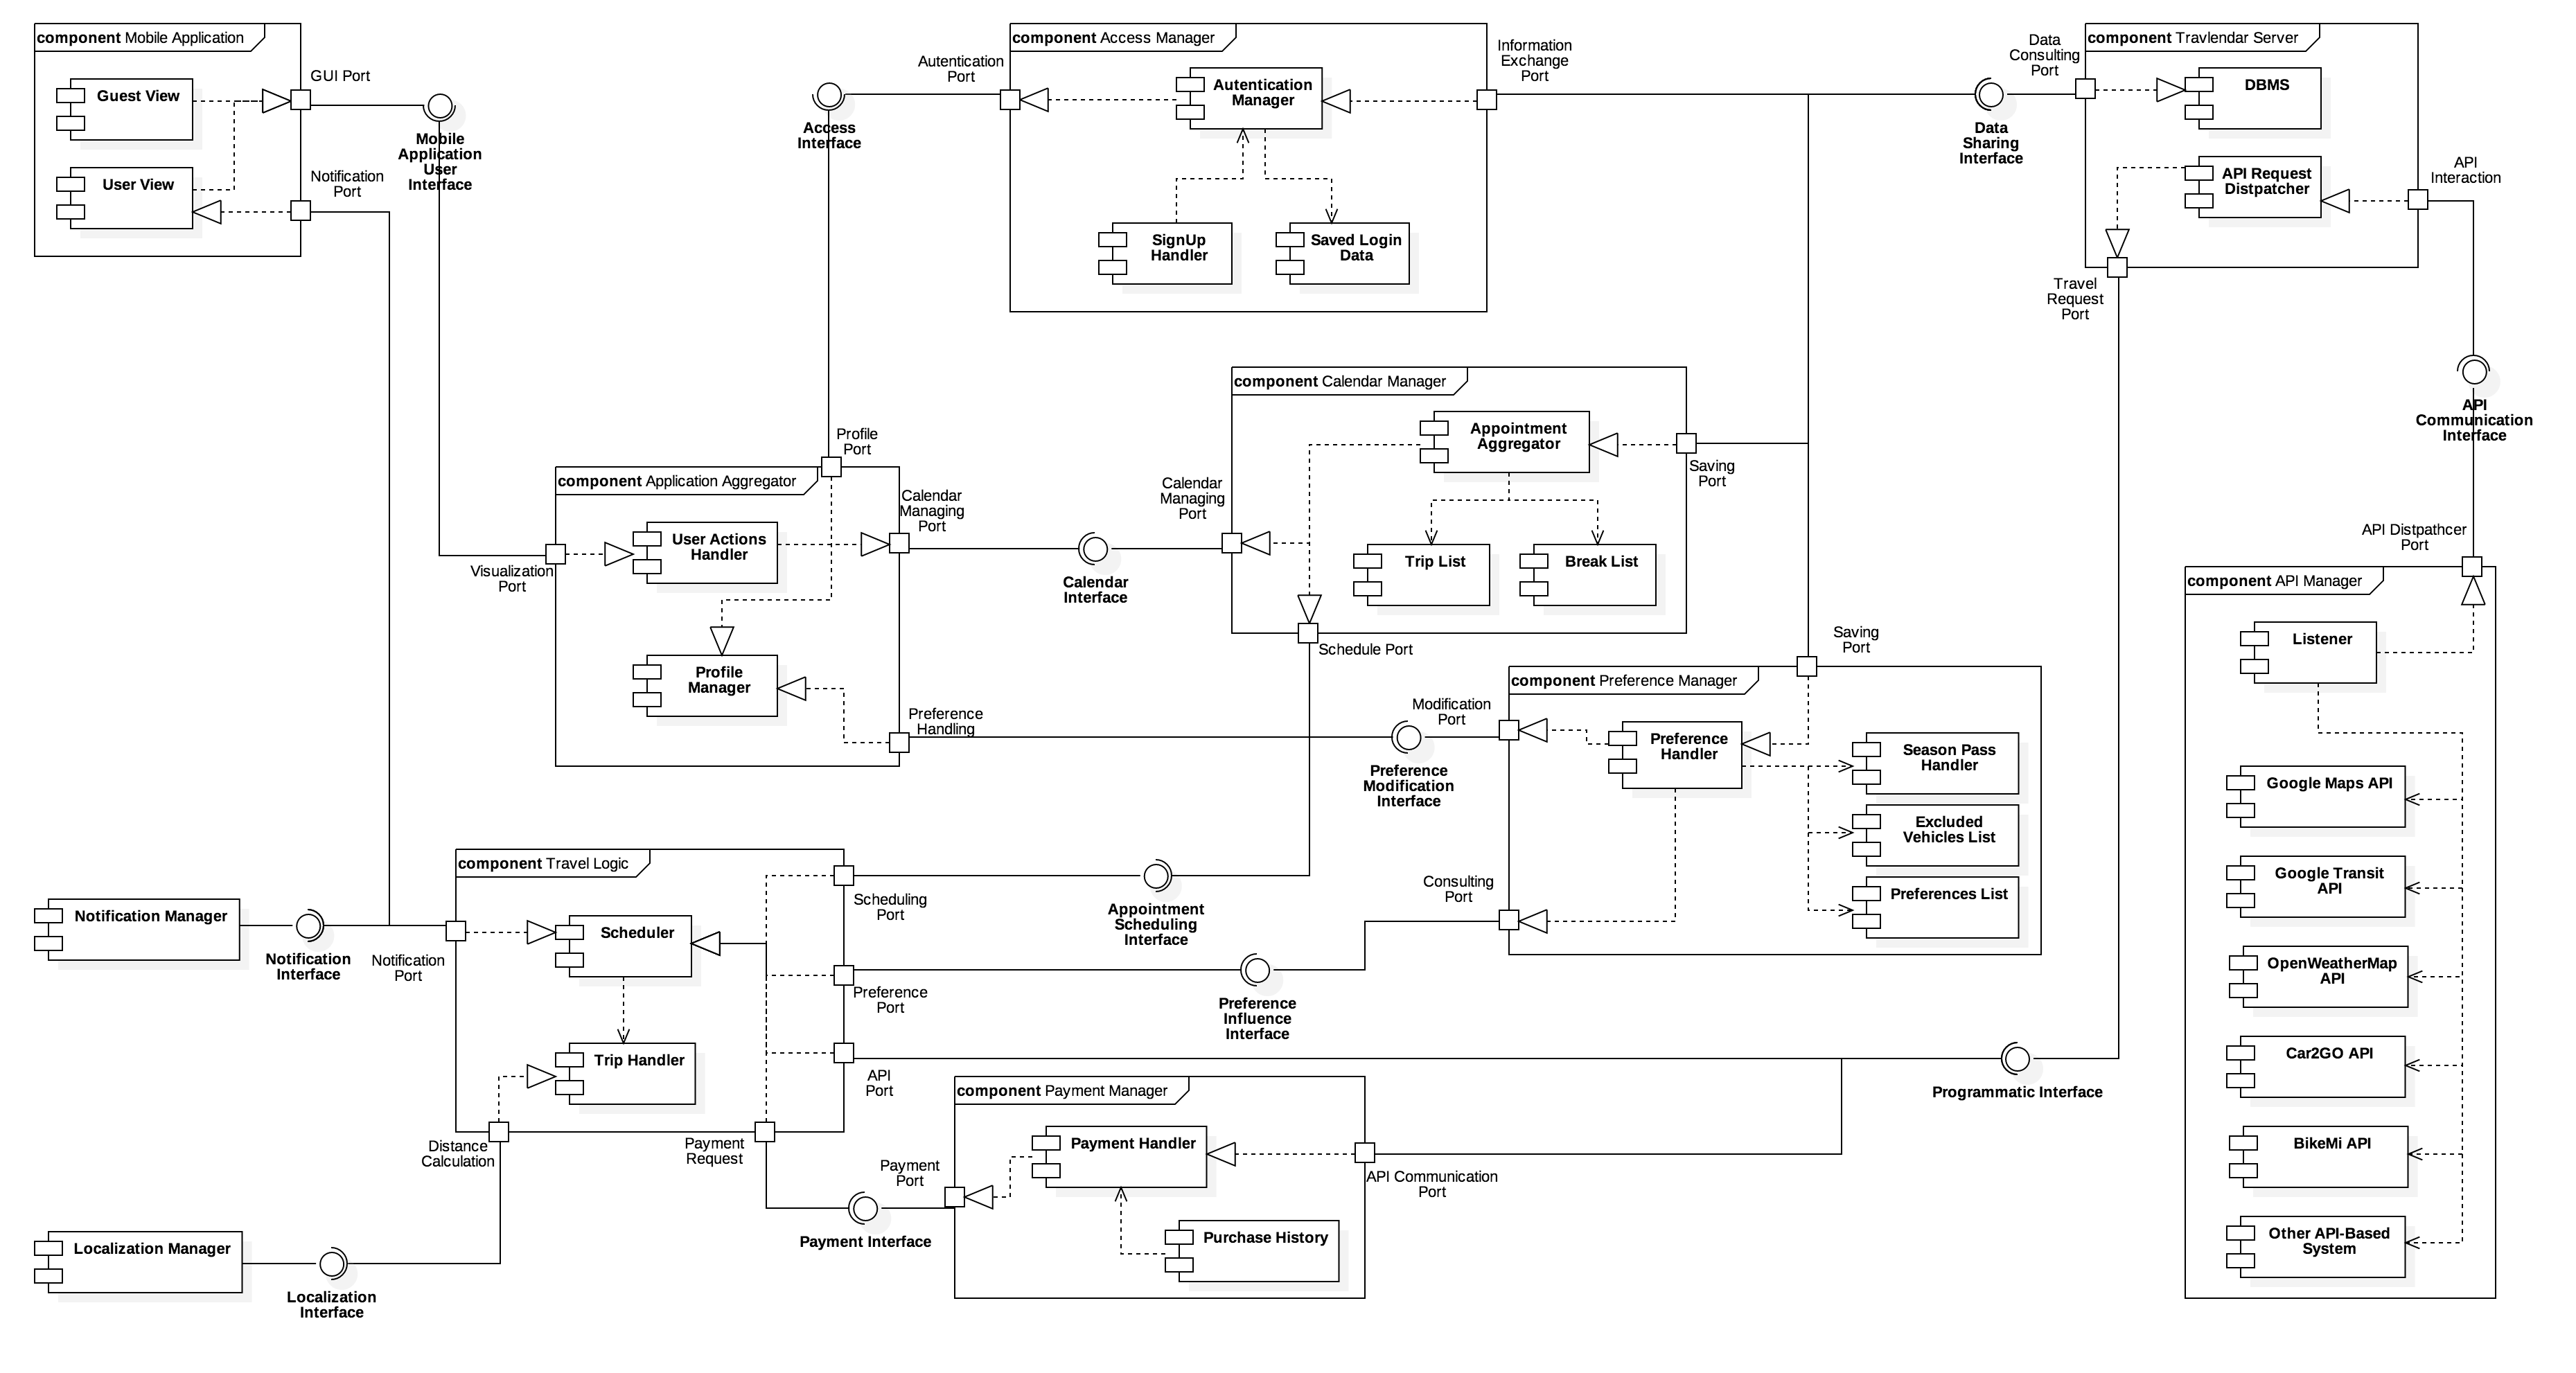
\includegraphics[height= 0.9\textheight]{UML/componentDiagrams/detailedLevel}
		\caption{Detailed level view}
		\label{detailedHighLevel}
	\end{figure}
\end{landscape}





	
\subsection{Deployment View}
	%The Component Diagram shown below describes the logical components of the system we are to develop, from a very high-level description on to a more detailed one. This diagram does not take into account the deployment phase, hence it doesn’t describe the logical layer of the system in terms of the physical tiers where it is deployed.

\begin{figure}[H]
		\centering
		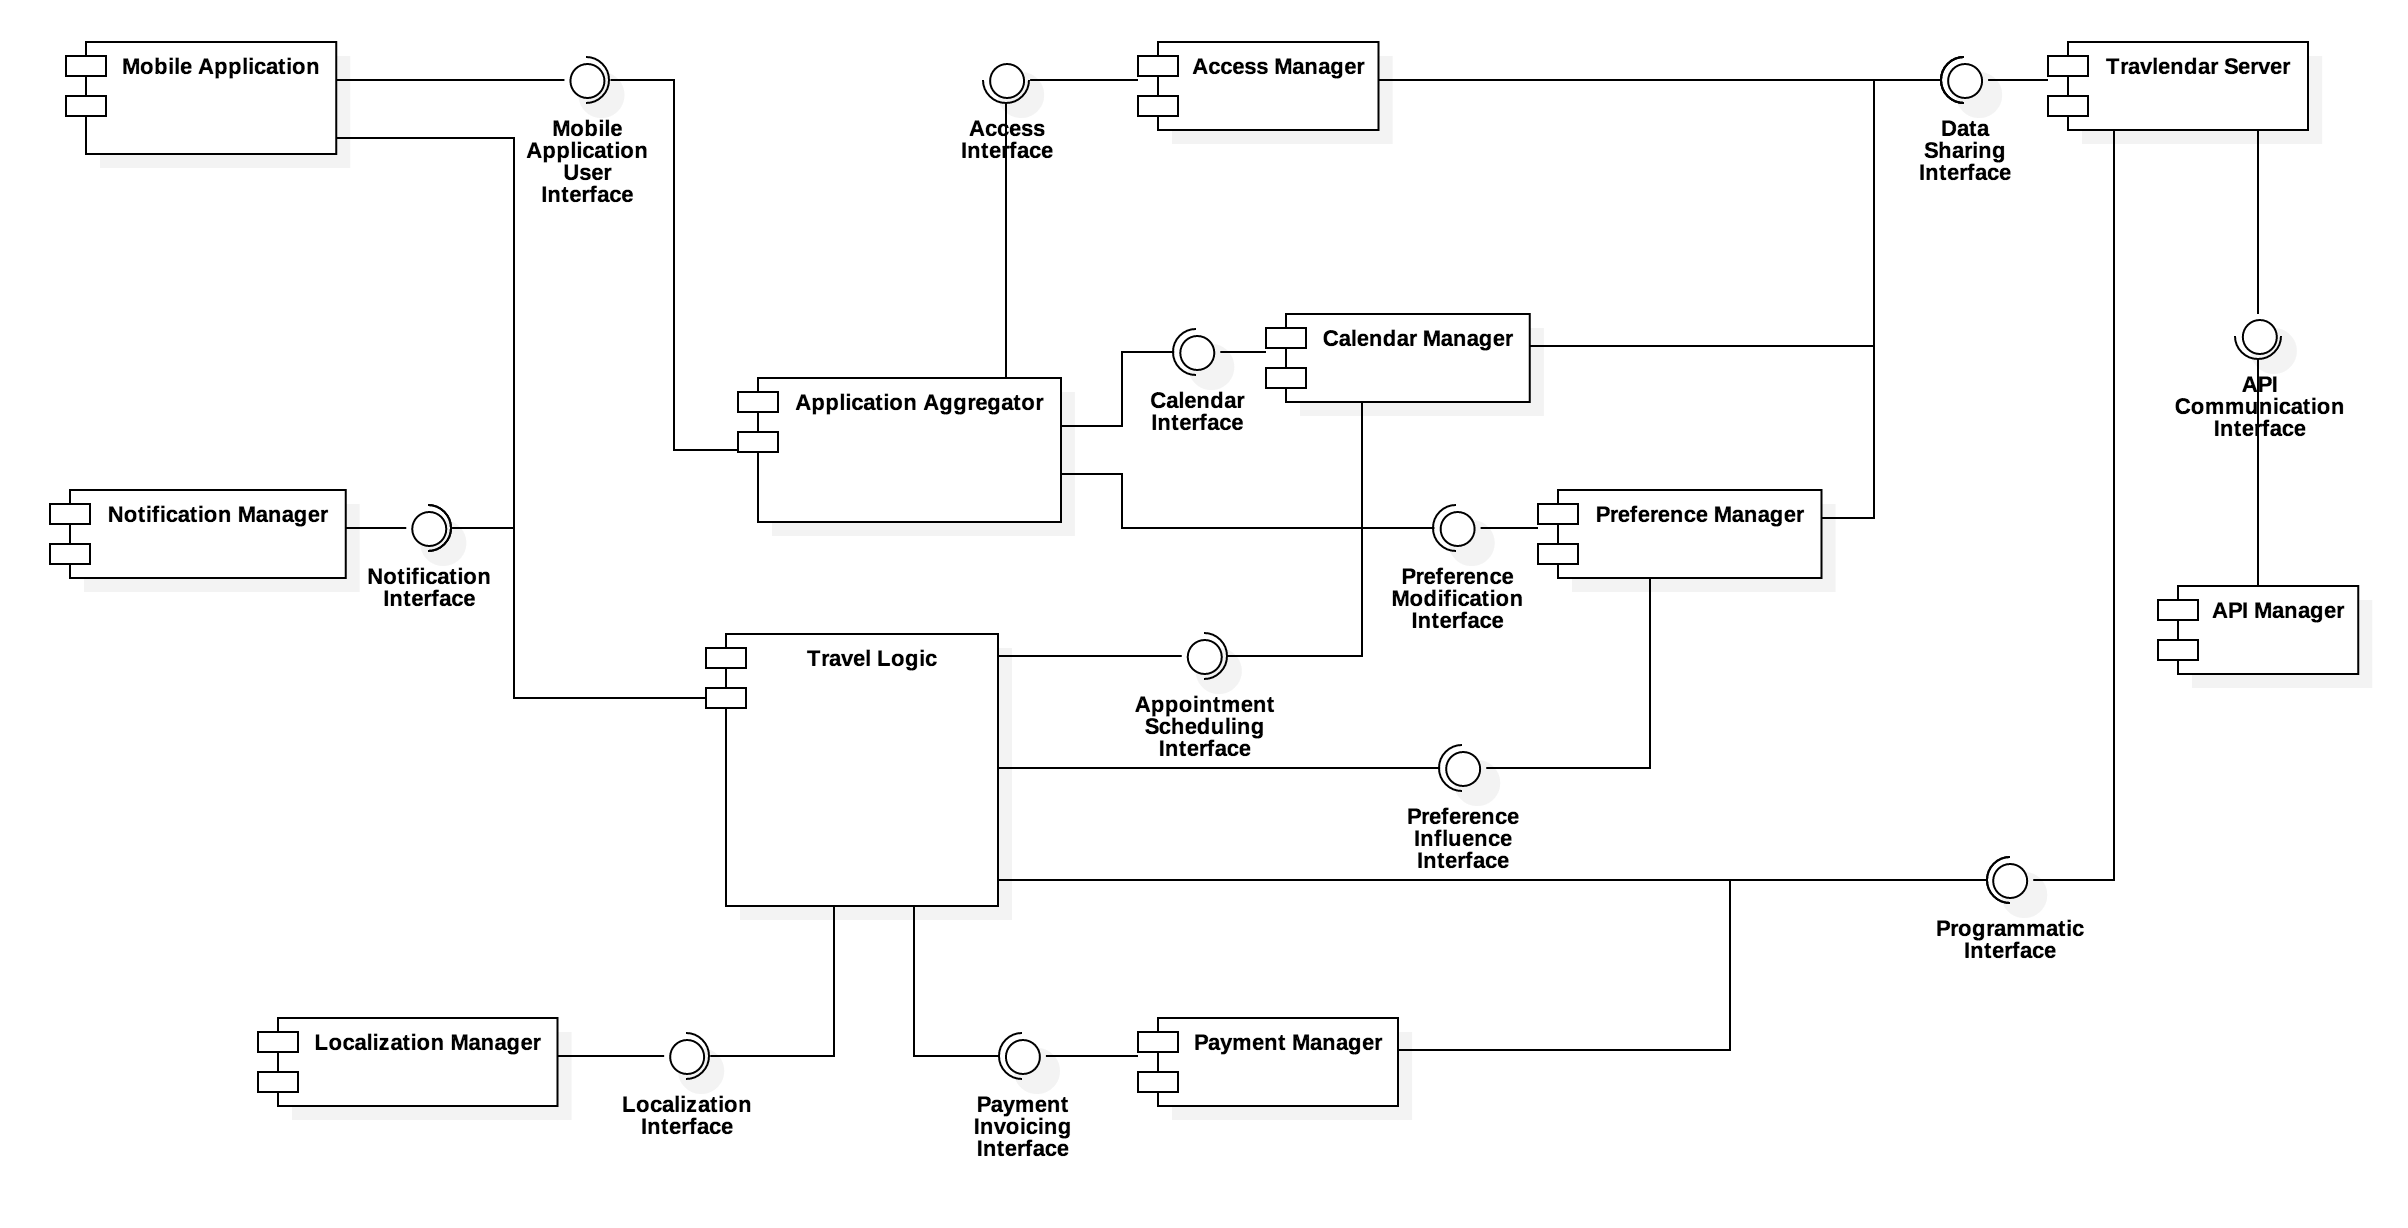
\includegraphics[width = \textwidth]{UML/componentDiagrams/highLevel}
		\caption{High level view}
		\label{componentHighLevel}
	\end{figure}

\paragraph{Mobile Application}
	This component represents the view of the User over its system. It’s split in two sub-components, Guest-view and User-view, which represents the two different ways an human interaction can be instaurated with the system.

	\begin{figure}[H]
		\centering
		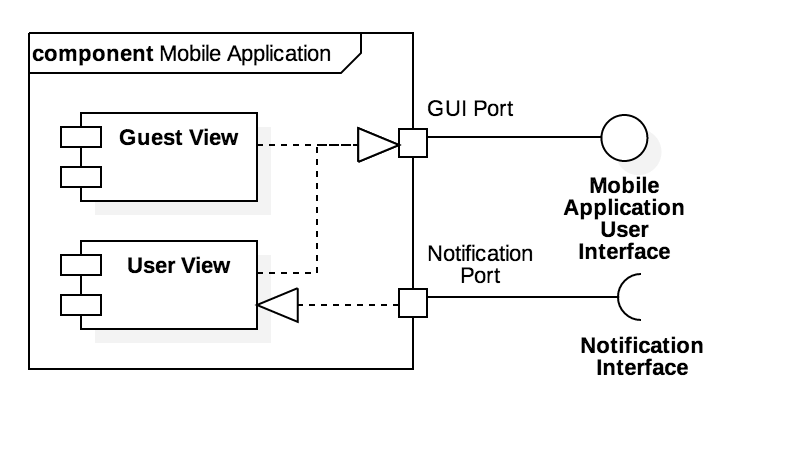
\includegraphics[scale = 0.2]{UML/componentDiagrams/mobileApplication}
	\end{figure}


\paragraph{Application Aggregator}
	This component works, unsuprisingly, as a collector of the different information \textit{Travlendar+} manages. It allows an easy management of every piece of information and allows us to avoid an high number of interfaces among the different components. 'Profile Manager' specifies the profile setting of the current user, while 'User Action Handler' allows us to register User's input.
	
	\begin{figure}[H]
		\centering
		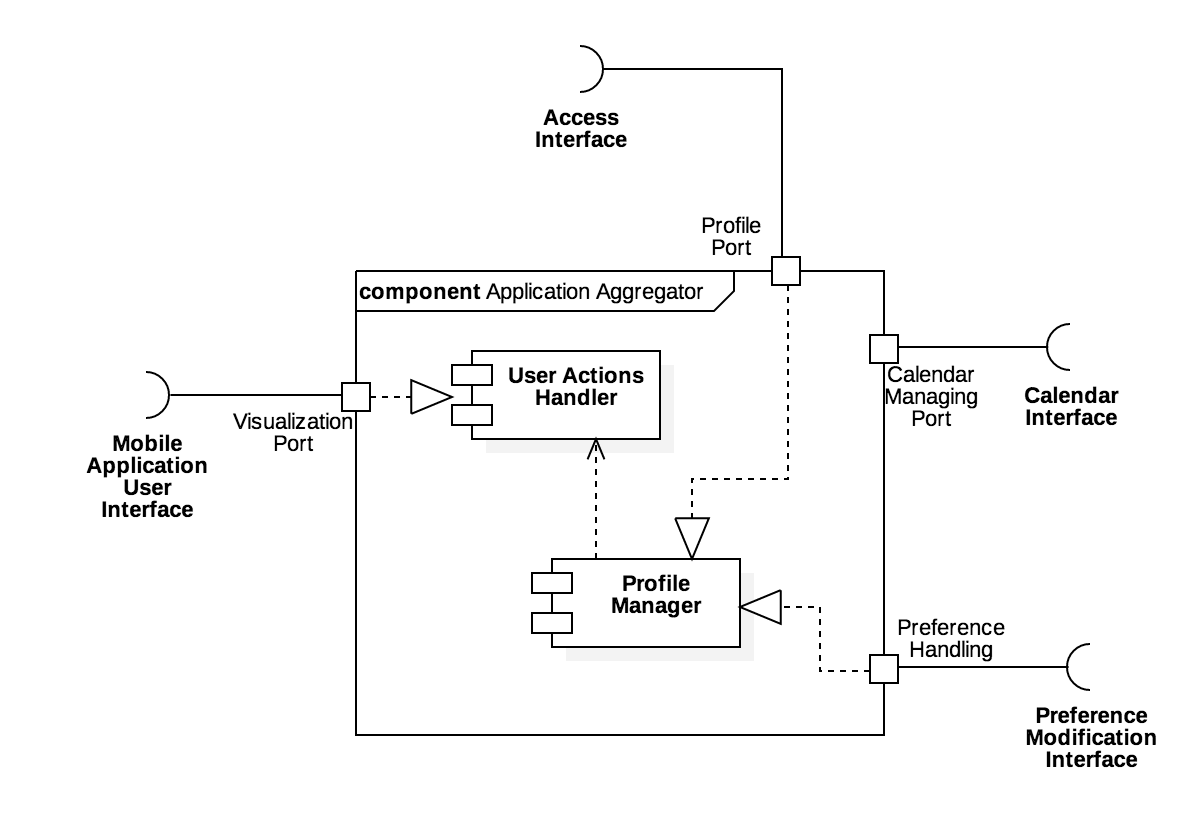
\includegraphics[scale = 0.2]{UML/componentDiagrams/applicationAggregator}
	\end{figure}
 
\paragraph{Calendar Manager}
	This component is divided into 'Appointments' and 'Breaks' sub-components, which track the appointments inserted by the User together with his breaks, and 'Trips', which is the list of trips arranged by the scheduler for every appointment. The sub-component 'Appointment Aggregator' serves the purpose of listing and presenting the content of the other two sub-components.
	
	\begin{figure}[H]
		\centering
		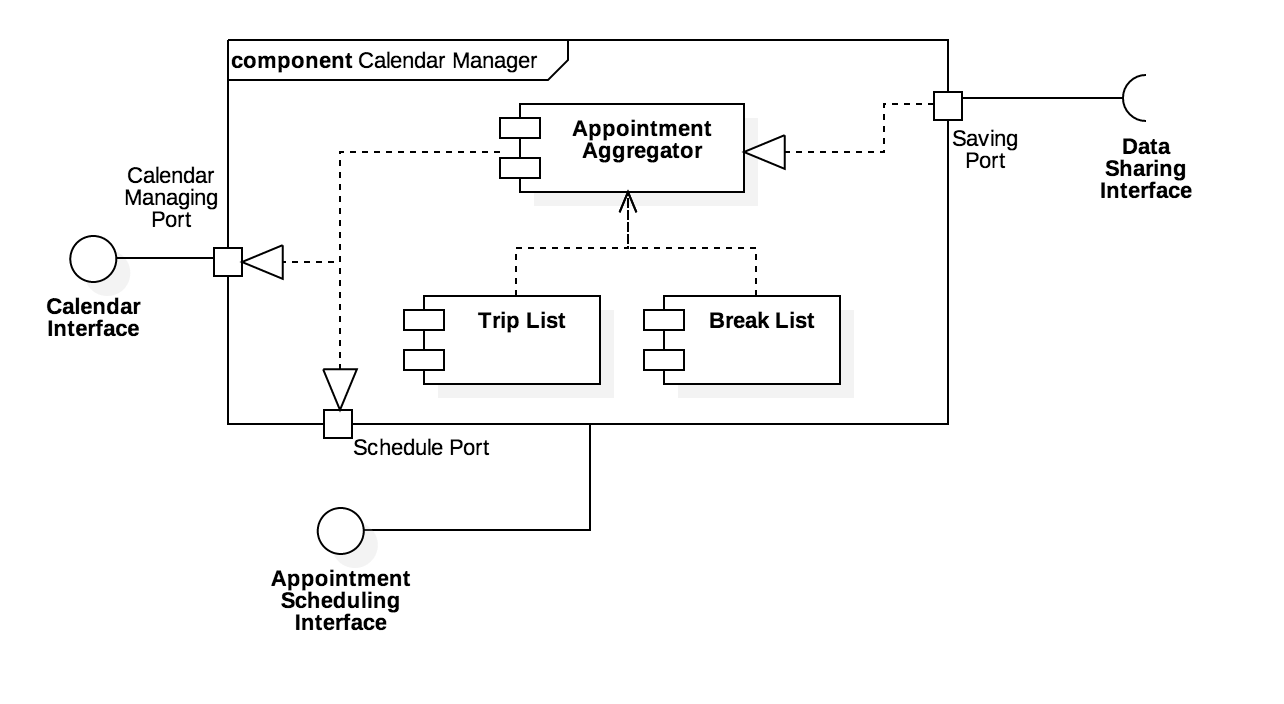
\includegraphics[scale = 0.2]{UML/componentDiagrams/calendarManager}
	\end{figure}
 

\paragraph{Preference Manager}
	This component serves the purpose of keeping track of the preferences expressed by the User. 'Season Pass Handler' takes care of storing season passes; 'Excluded Vehicles List' cuts off from the scheduler results involving a selection of banned transportation means, 'Preferences List' covers the remaining and wider spectrum of User's choices. 'Preference Handler' is the sub-component that manages the other ones and that communicates outside Preference Manager.

	\begin{figure}[H]
		\centering
		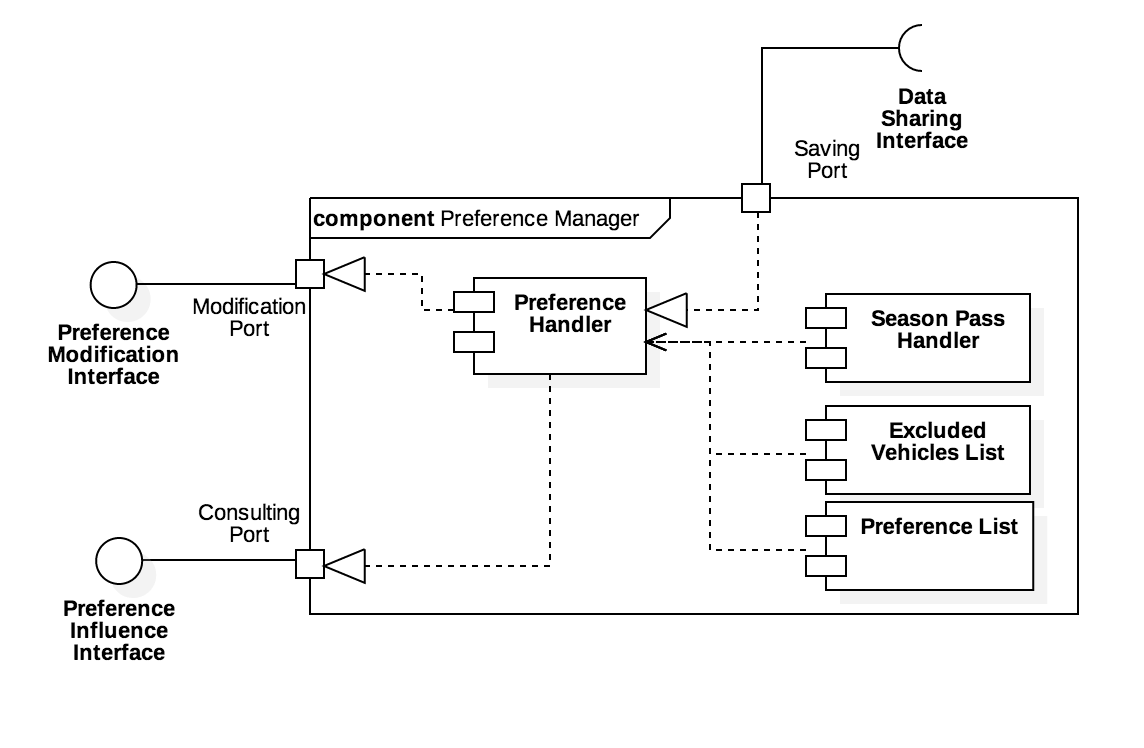
\includegraphics[scale = 0.2]{UML/componentDiagrams/preferenceManager}
	\end{figure}
	

\paragraph{Travlendar Server} 
	This component represents the \textit{Travlendar Server} whose purpose is to store User's preferences, access data and personal information. It is modeled by its 'DBMS' component, which stores Timetables and Preferences and the 'API Request Dispatcher', which forwards requests to external agents.

	\begin{figure}[H]
		\centering
		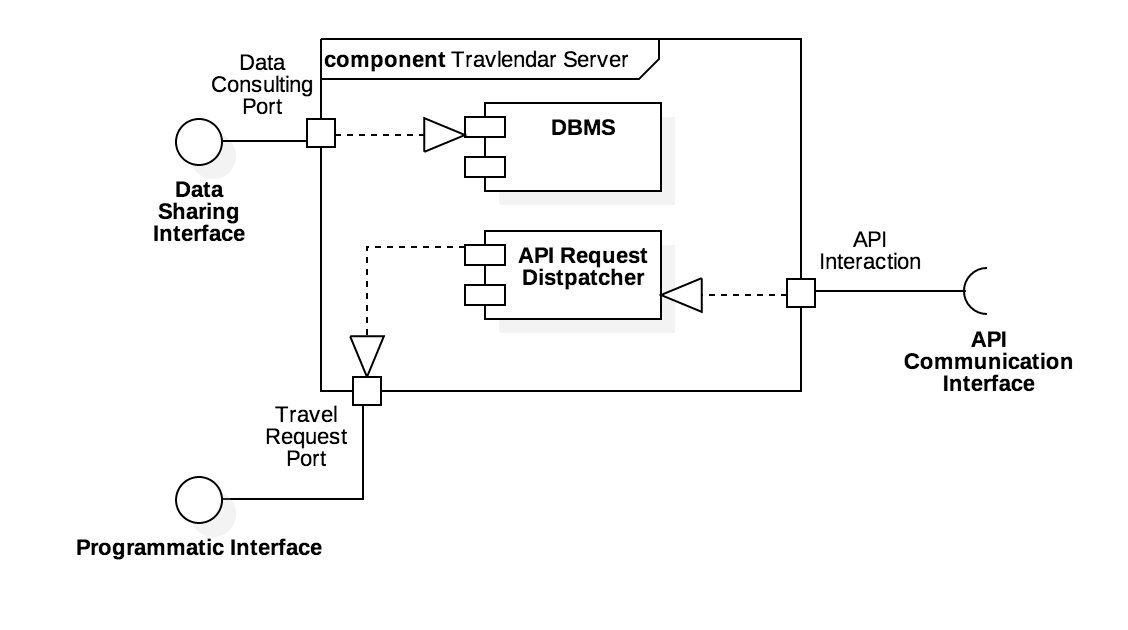
\includegraphics[scale = 0.2]{UML/componentDiagrams/travlendarServer}
	\end{figure}
	

\paragraph{Travel Logic Manager}
	This component is split into two sub-components: 'Scheduler' is the fundamental block that aims at scheduling and arranging User appointments and breaks via the the corresponding trips, 'DistanceManager' is the block whose purpose is to organize and present travel times to the scheduler in order to have them sorted out and well-managed.

	\begin{figure}[H]
		\centering
		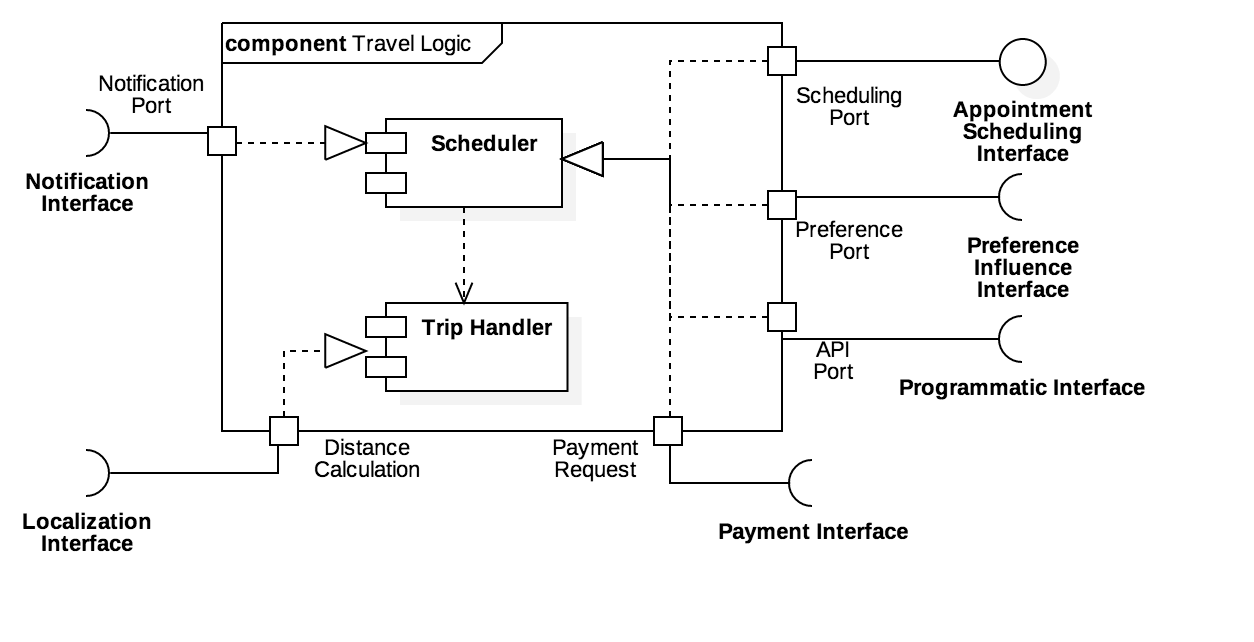
\includegraphics[scale = 0.2]{UML/componentDiagrams/travelLogic}
	\end{figure}
	

\paragraph{Payment Manager}
	This component deals with the recording of purchases and their associated credit cards.
	The sub-component 'Payment Handler' tracks purchase records and interacts with the required apps installed on the mobile device, while 'Purchase History' is an exploitable and rational organizations of the credit cards used by the user.

	\begin{figure}[H]
		\centering
		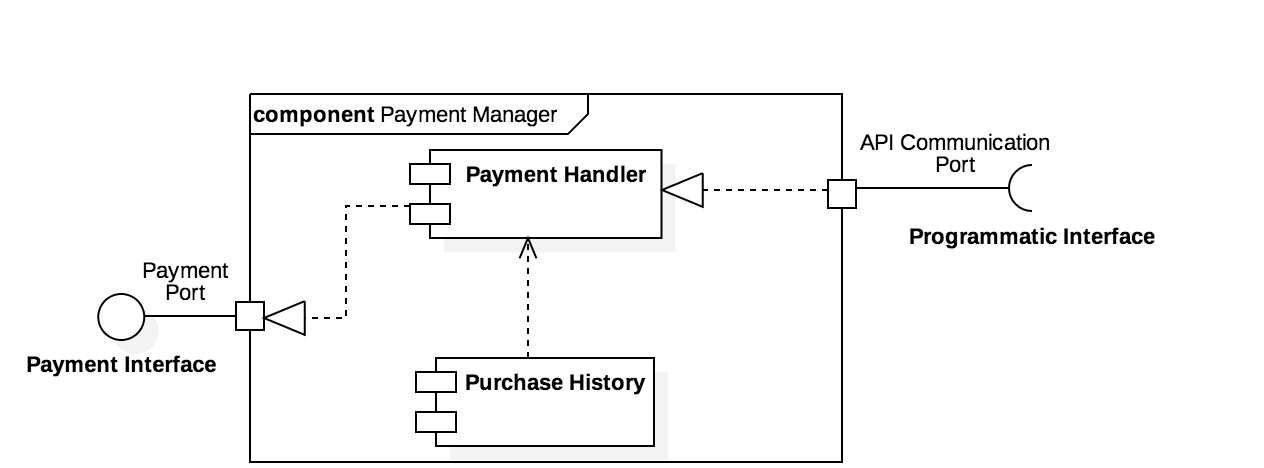
\includegraphics[scale = 0.2]{UML/componentDiagrams/paymentManager}
	\end{figure}
	

\paragraph{API Manager} 
	This component is critical in order to provide a functioning Travel Logic: it gathers the interactions with all external APIs.
	Here are listed the APIs the mobile application project starts with : Google Maps API, Google Transit API, Open Weather Map API, Car2Go and BikeMi API.
	The last couple is for reference only, as already pointed in the RASD. Naturally, the list of external services can be expanded.
	The 'Listener' component serves the purpose of forwarding requests and receives the desired inputs.
	
	\begin{figure}[H]
		\centering
		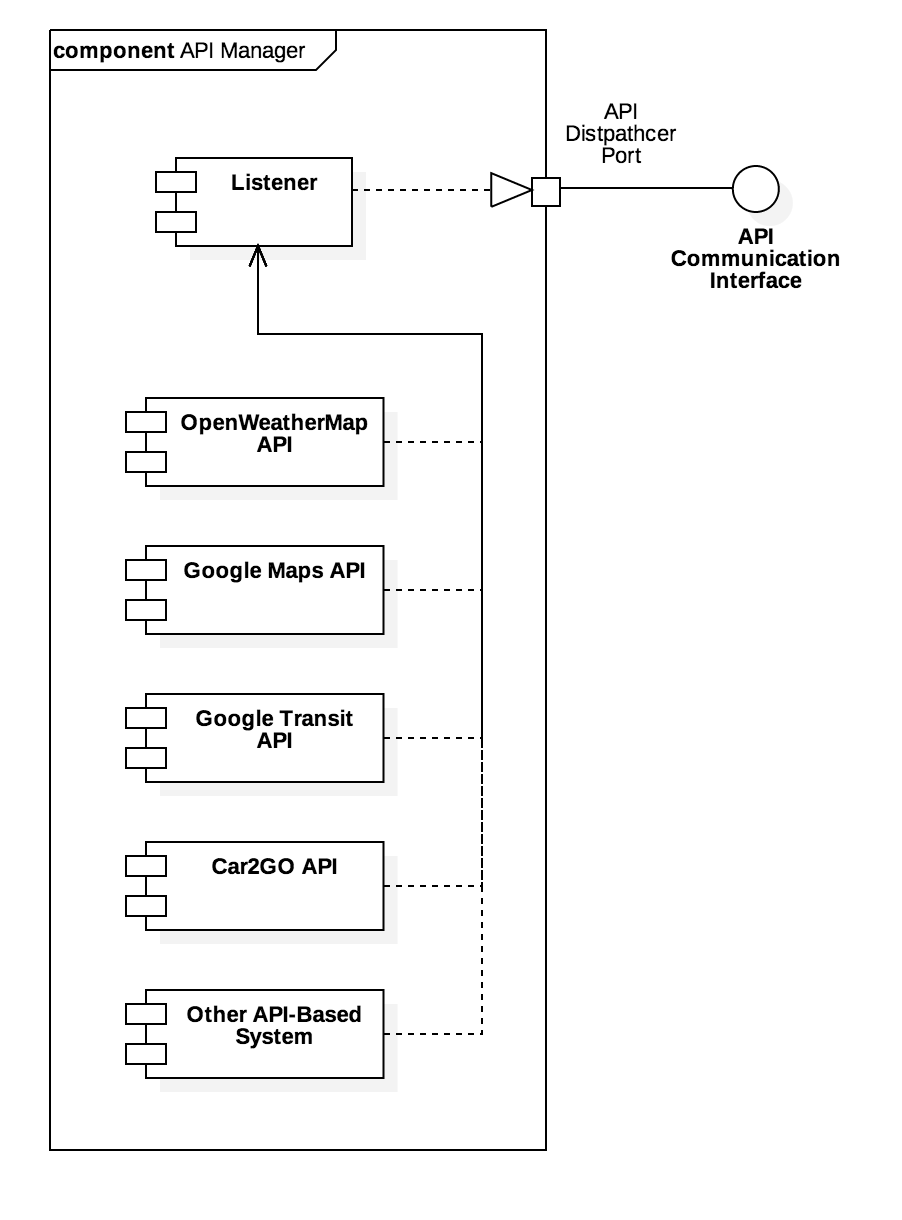
\includegraphics[scale = 0.2]{UML/componentDiagrams/APIManager}
	\end{figure}
	
	
\paragraph{Notification Manager}
	This component allows the notification system to warn users in the cases events partially or completely overlap according to the scheduler.

\paragraph{Localization Manager}
	This component represents the localization functionalities of the mobile application.
	
\begin{landscape}
	\begin{figure}
		\centering
		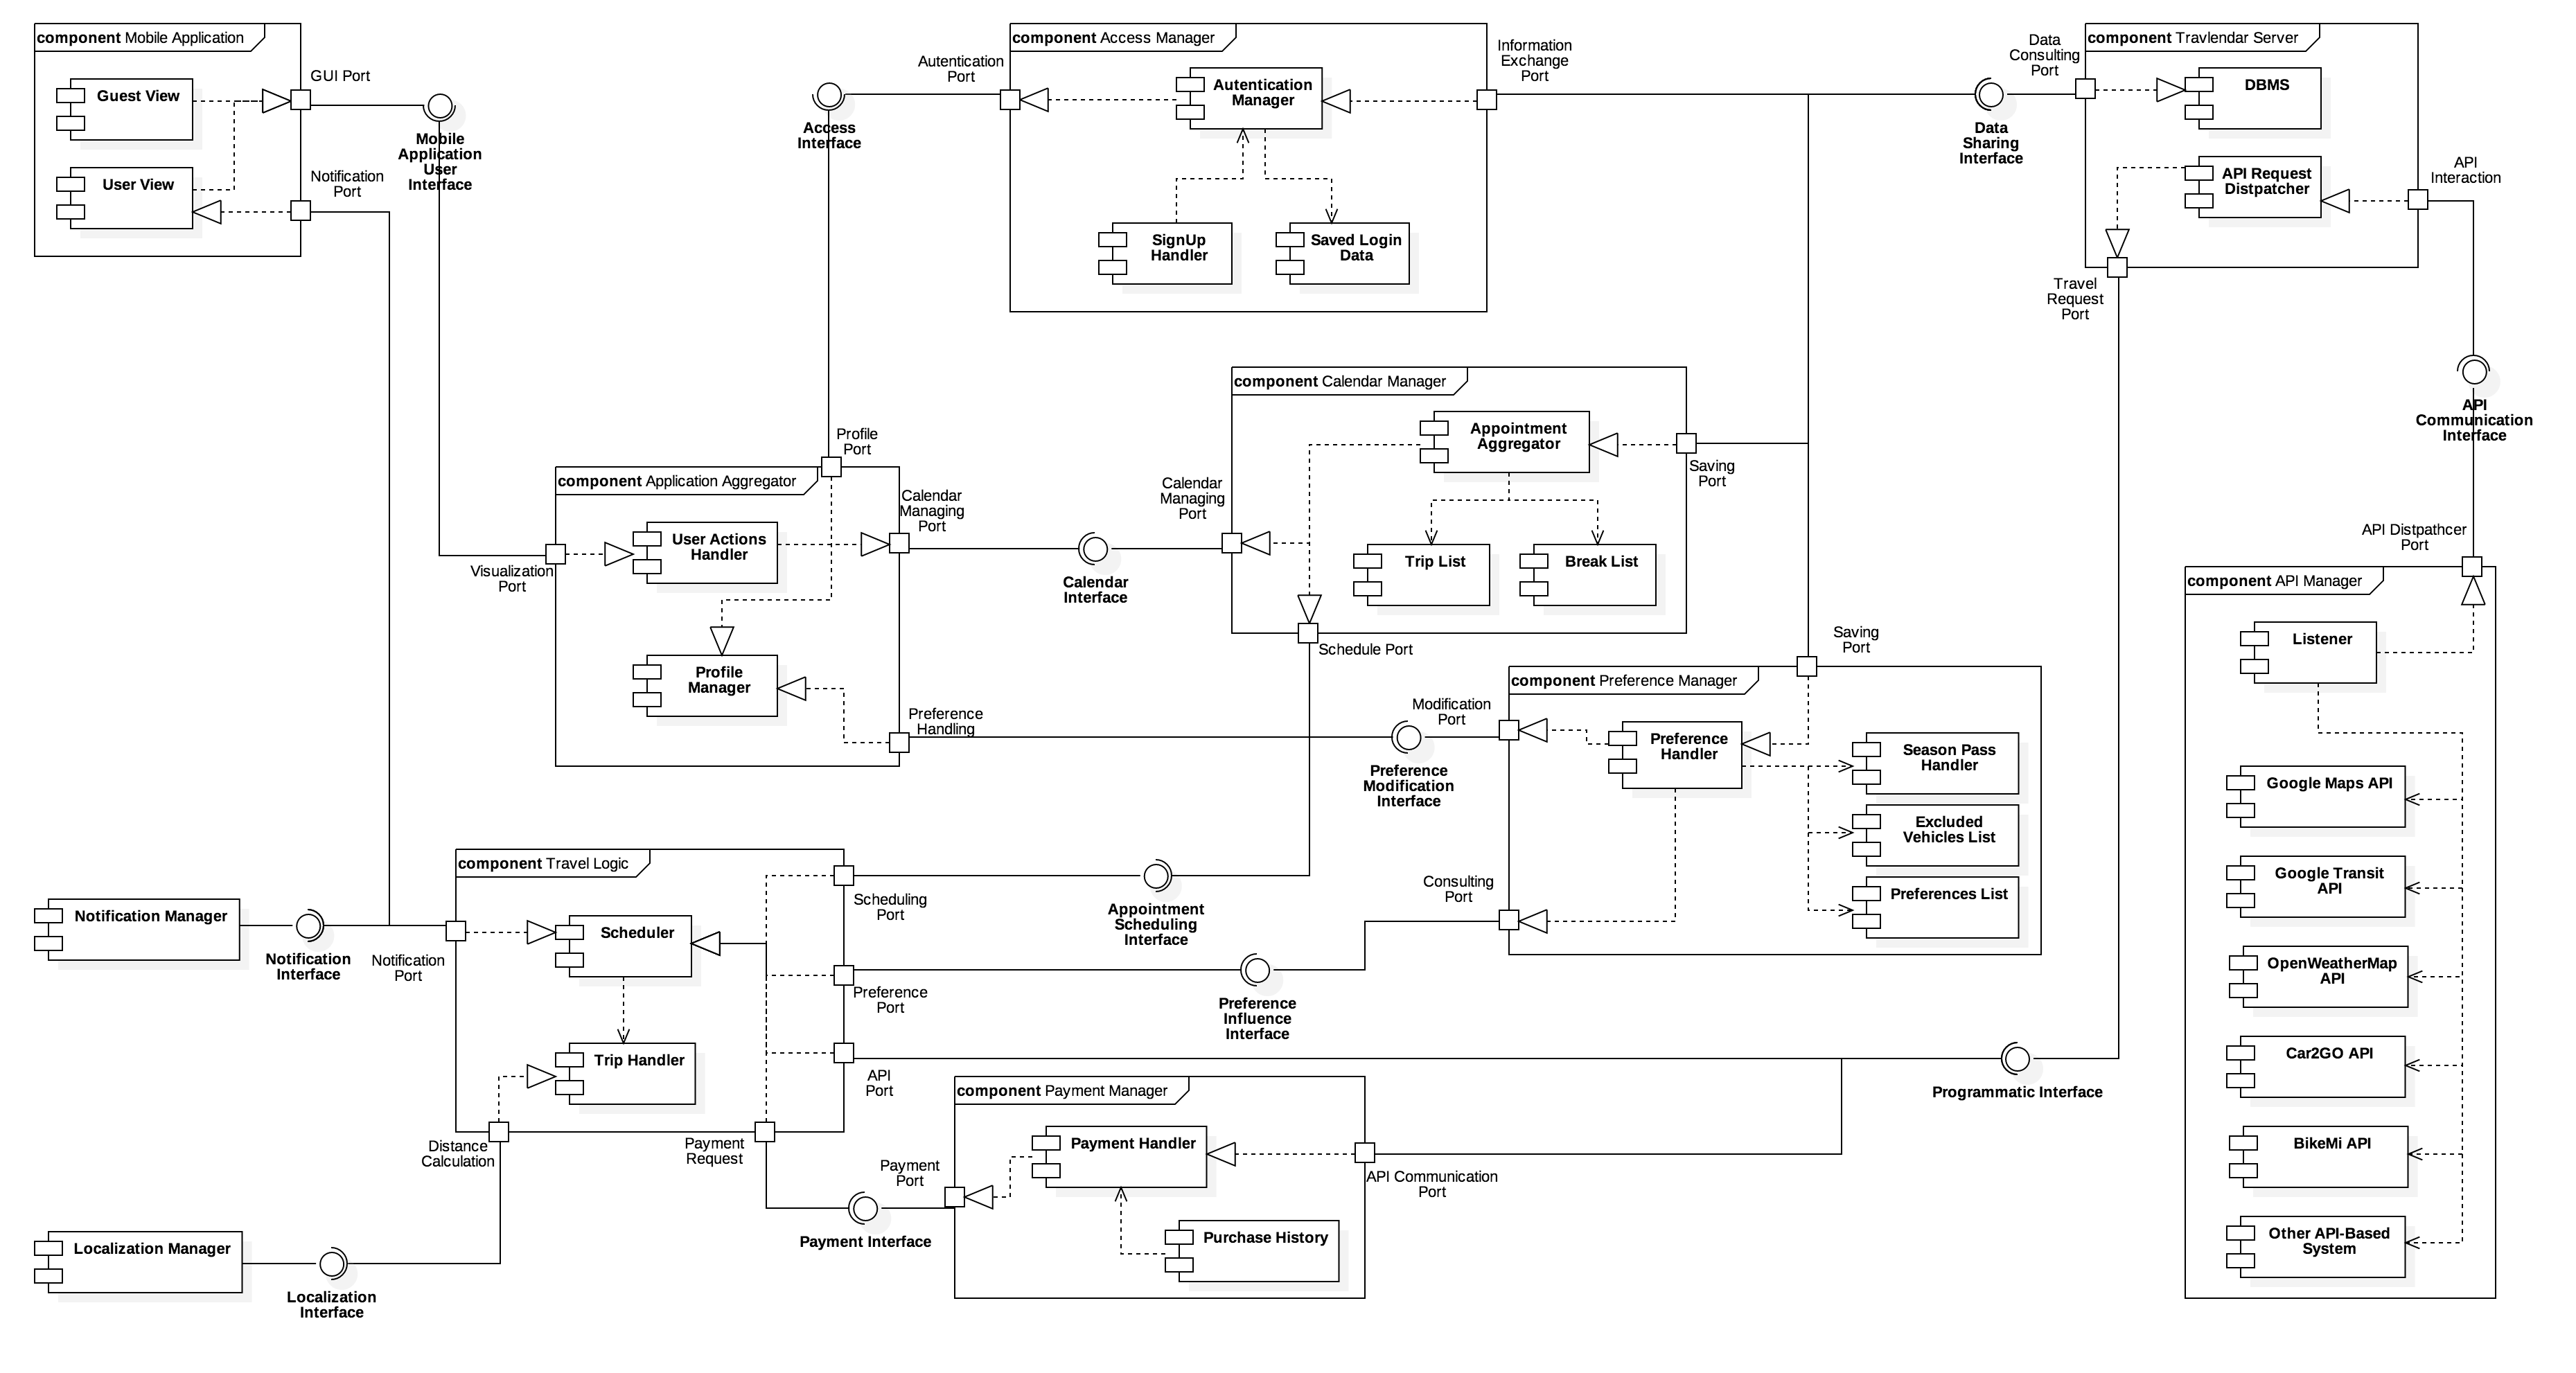
\includegraphics[height= 0.9\textheight]{UML/componentDiagrams/detailedLevel}
		\caption{Detailed level view}
		\label{detailedHighLevel}
	\end{figure}
\end{landscape}





	
\subsection{Runtime view}
	%\input{subsections/section2/rutimeView.tex}

\subsection{Component Interfaces}
	%In this section we will show the component Interfaces. For each one are reported the main functionalities.
Nevertheless we need to keep in mind that in further implementations these functions can be splitted into less complex ones.

\begin{figure}[H]

	\begin{subfigure}[t]{0.3\linewidth}
		\centering
		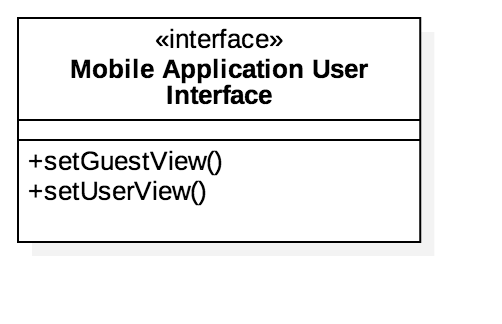
\includegraphics[width=\linewidth]{UML/Interfaces/mobileApplicationUserInterface}
		\caption{Mobile Application User Interface}
	\end{subfigure}
	~
	\begin{subfigure}[t]{0.3\linewidth}
		\centering
		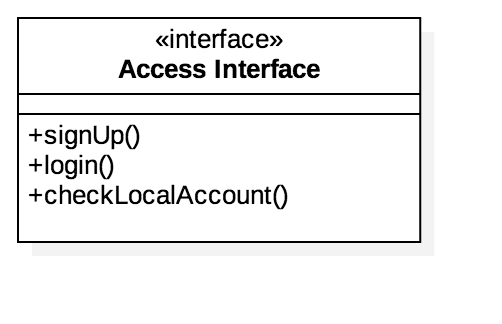
\includegraphics[width=\linewidth]{UML/Interfaces/accessInterface}
		\caption{Access Interface}
	\end{subfigure}
	~	
	\begin{subfigure}[t]{0.3\linewidth}
		\centering
		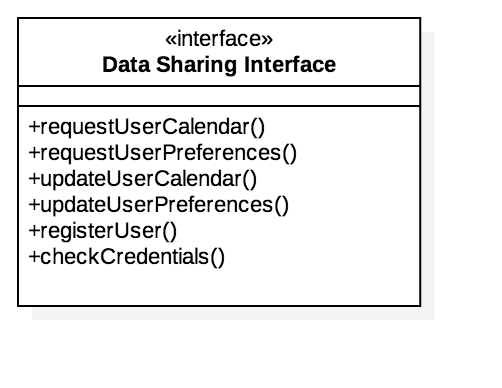
\includegraphics[width=\linewidth]{UML/Interfaces/dataSharingInterface}
		\caption{Daba Sharing Interface}
	\end{subfigure}
	\hfill
	\vskip0.75cm
	
	
	\begin{subfigure}[t]{0.3\linewidth}
		\centering
		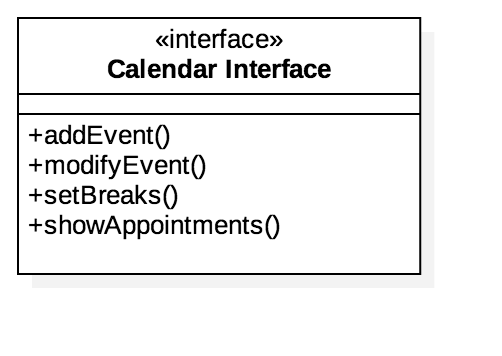
\includegraphics[width=\linewidth]{UML/Interfaces/calendarInterface}
		\caption{Calendar Interface}
	\end{subfigure}
	~
	\begin{subfigure}[t]{0.3\linewidth}
		\centering
		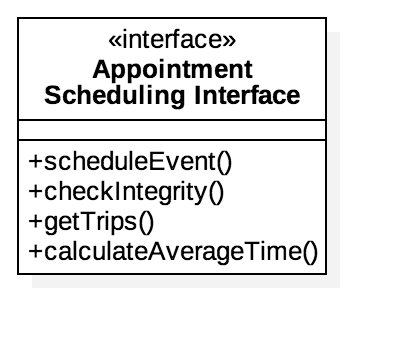
\includegraphics[width=\linewidth]{UML/Interfaces/appointmentSchedulingInterface}
		\caption{Appointment Scheduling Interface}
	\end{subfigure}
	~
	\begin{subfigure}[t]{0.3\linewidth}
		\centering
		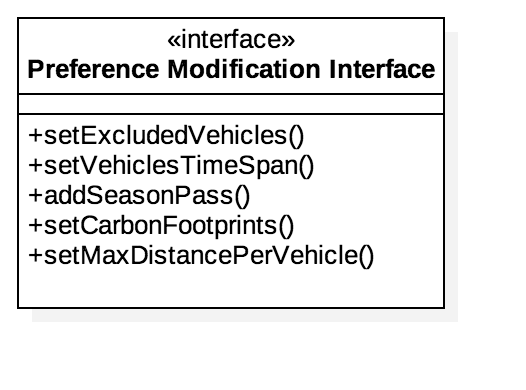
\includegraphics[width=\linewidth]{UML/Interfaces/preferenceModificationInterface}
	\caption{Preference Modification Interface}
	\end{subfigure}
	\hfill
	\vskip0.75cm
	
	
	\begin{subfigure}[t]{0.3\linewidth}
		\centering
		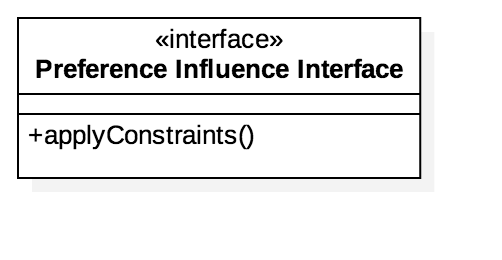
\includegraphics[width=\linewidth]{UML/Interfaces/preferenceInfluenceInterface}
		\caption{Preference Influence Interface}
	\end{subfigure}
	~
	\begin{subfigure}[t]{0.3\linewidth}
		\centering
		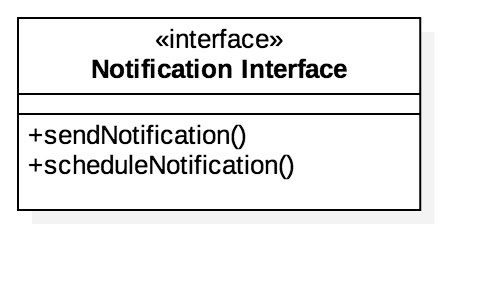
\includegraphics[width=\linewidth]{UML/Interfaces/notificationInterface}
		\caption{Notification Interface}
	\end{subfigure}
	~
	\begin{subfigure}[t]{0.3\linewidth}
		\centering
		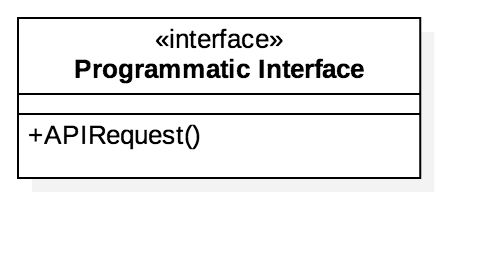
\includegraphics[width=\linewidth]{UML/Interfaces/programmaticInterface}
		\caption{Programmatic Interface}
	\end{subfigure}
\end{figure}	


\begin{figure}[H]\ContinuedFloat
	\begin{subfigure}[t]{0.3\linewidth}
		\centering
		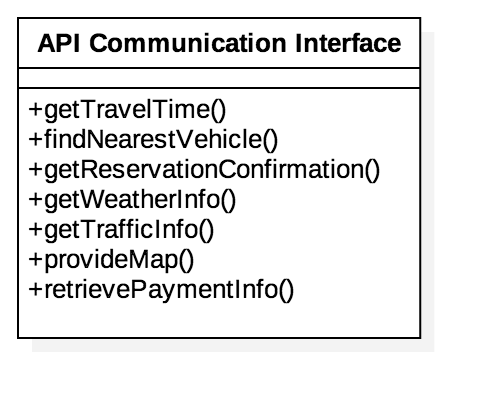
\includegraphics[width=\linewidth]{UML/Interfaces/APICommunicationInterface}
		\caption{API Communication Interface}
	\end{subfigure}
	~
	\begin{subfigure}[t]{0.3\linewidth}
		\centering
		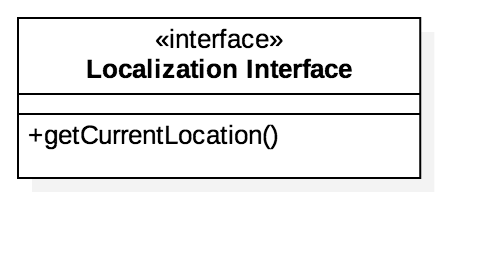
\includegraphics[width=\linewidth]{UML/Interfaces/localizationInterface}
		\caption{Localization Interface}
	\end{subfigure}
	~
	\begin{subfigure}[t]{0.3\linewidth}
		\centering
		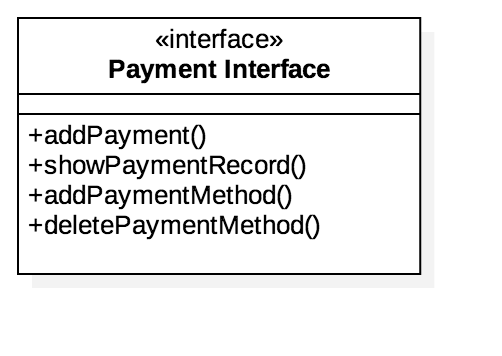
\includegraphics[width=\linewidth]{UML/Interfaces/paymentInterface}
		\caption{Payment Interface}
	\end{subfigure}
	
	\caption{List of Interfaces}
\end{figure}

\subsection{Architectural Styles}
	
[Architectural Style]

For our system architecture we adopt a 3-tier client/server architecture : we'll have a Mobile Application Clients, a Travlendar
 Server and a Data Storage Layer.


Mobile Application Clients : This layer is represented by the Travlendar+ Application, a thick client and an interactive and dinamic GUI.
The application will be written in Java for increased portability and will be able both to geo-localize its user and to communciate with the core of the travel : this is the foundation of information synching and requests forwarding to APIs.

Travlendar+ Server : The business Server runs the business logic. Its main duty is to forward requests of the users to the Data layer and external APIs while saving all necessary users' preferences and timetables. These operations are executed under a microservice architectural pattern.

The Data Layer : This layer comprehends both the DBMS which stores and manages users' preferences and timetables and the external service agents (objects which call external services). In the former case it is required the capability of providing data through SQL queries using ODBC protocol, while in the latter it is required a good implementation of the ad-hoc functions of the external APIs.
(link Microsoft)

Patterns

Pattern are mostly required to smooth the construction of our system. In particular, we'll be using a MVC (Model - View - Control) Pattern for our mobile application, Adapter (??), Client/Server and Single Instance component.

MVC is used to define our Java mobile application : the view will be the dynamic GUI, the Travel Logic the control and the model will be the data received from the APIs and the locally stored timetables and trips.


Single Instance component will be mostly useful when treating the components of the mobile application : components like Access Manager or Travel Logic will be the ones mainly touched by this pattern.

Client/Server pattern is the one we adopted to shape the interactions between our mobile application (the client) and the Travlendar+ Server (i.e, the server). Reasons for adoption have mainly been the simplicity and widespread use of the model.


%Vecchia parte di Michele!
In particolare ci serviremo del pattern MVC (Model View Control) molto utile perchè ci permette di separare la logica Business dalla logica di Presentazione. In questo caso il Database interpreterà il ruolo del Model, Mobile Application interpreterà il ruolo di View, e il Server sarà il Control. 

		
%%% 3 -ALGORITHM DESIGN  %%%
	\newpage
	\section{Algorithm Design}
		% RANK SOLUTIONS %
\paragraph{solution Ranking}
This algorithm shows how System ranks all the feasible solution based provided by the external sources, like Public Transportation, via Car, Bike or Foot, depending on:
	\begin{itemize}
		\item[•] time needed for completing the trip.
		\item[•] number of subtrips (only for Public Tranportation).
		\item[•] if the Car have to be used in other trips on that day.
		\item[•] money needed for the Tranportation Mean, calculated as:
			\begin{itemize}
				\item[-] public ticket cost for Public Services.
				\item[-] average fuel cost for Car.
				\item[-] tariff \euro /time for Sharing services.
			\end{itemize}
		\item[•] User preferences.
		\item[•] Weather forecast for the Appointment day (if and only if the Appointment is no longer than 15 days).
	\end{itemize}
	
	Since solutions have been already calculated individually, is supposed that every element in the input list has been already divided in subtrips either by the External API Manager or by Scheduler (see figure \ref{travelLogicDetail} and figure \ref{APIManagerDetail}) in a previous Step.
	Is also assumed that 'Public Service Manager' (see RASD Class Diagram) provides a list of different tranportation means, and all the consistent possible combinations of them.
	
	First of all Every element in the input list is filtered by the 'Excluded Vehicles List' (see figure \ref{preferenceManagerDetail})
	For remaining elements, every inner SubTrip time is compared with the average reference time that the User have to spend by going with owned Car or bike, or, if is a short distance, by going with foot, in order to categorize solutions in \textit{suitables}, \textit{valid alternatives}, and \textit{unconvenient}.
	
	
	
	Then for every category solutions:
	\begin{itemize}
		\item[-] items are orderd by \textit{time needed} and \textit{number of SubTrip}
		\item[-] if User has a Season Pass of a public transportation company, relative solutions are put on the highest rank.
		\item[-] solution cost are calculated, as aforementioned.
	\end{itemize}		
		
	If a solutions from lower category are advantageous with respect to 'higher' solutions, those are put again in the upper category.
	A solution is advantageous if \textit{time needed}s difference between the two category, defined as 
	\\ \quad $\Delta =  timeNeeded(bestUpperSolution) - timeNeeded(lowerSolution)$, \\
	is less than 15 minutes, and either is a cheaper solution or User has a Season Pass that doesn't belong to any other company of Upper-category solutions.
		
	If the Appointment is scheduled in less than 15 days, and weather forecast is predicted al \textit{non consistent for outdoor tripping}, solutions that expect a $total\_Outdoor\_Time$ defined as the sum of the time spent by walking and biking, greater than 3 minutes are downgraded in the respective category.

	If in the other Appointments of that day a proprietary Car solution is already scheduled, 'Only by Using Car' solution will be encouraged, but if and only if:

	In the end all the category \textit{suitables} and \textit{valid alternatives} are merged into an unique list made so that User can choose one.
	The algorithm return also the $bestSolution$ got by 'Poping' of the first element of the list, and the solution obtained by 'Only Walking' and 'Only by Using Car'.
	
	\vfill
	\begin{algorithm}[H]
\caption{Rank Solution}
	\KwData{Trip, List of Calculated Solutions, Preferences, Calendar}
	\KwResult{List of Ranked Solutions, Best Calculated Solution, Only Car Time, Only Walking Time}
		
	\bigskip
	\tcp{Calculate 'Only Car' and 'Only Walking' Solutions}
	$ carSolution \leftarrow \textbf{Scheduler}.carTime$\;
	$ bikeSolution \leftarrow \textbf{Scheduler}.walkingTime$\;
		
	\bigskip
	\tcp{Filtering Solutions based on $Preferences$}	
	\ForAll{Trip in Input\_List}{
		\If{Trip.AssignedTransportationMean() is in Excluded\_Vehicles\_List}{
			$ InputList.remove(Trip) $\;
		}
	}
	$ FilteredList \leftarrow InputList $\;

	\bigskip
	\tcp{Assign a category}	
	\ForAll{Trip in Filtered\_List}{
		$ \delta_{Advantage} \leftarrow 0$\;
		\ForEach{SubTrip in Trip}{
			\Switch{SubTrip}{
				\Case{Long\_Distance}{
					$ AVG\_Ref \leftarrow 
						\quad \arg\min
							\Big( \textbf{Scheduler}.AVG\_Time(Car), \textbf{Scheduler}.AVG\_Time(Bike) \Big)$\;
				}
				\Case{Short\_Distance}{
					$ AVG\_Ref = \textbf{Scheduler}.AVG\_Time(Foot)$\;
				}
			}
			$ comparison \leftarrow AVG\_Ref - SubTrip.Time$\;
			$ \delta_{Advantage} \leftarrow \delta_{Advantage} + comparison$\;
		}
			
		\bigskip
		\If{$ \delta_{Advantage} \gg 0 $ }{ 
			$ Suitable\_List.add(Trip)$\;
		}
		\ElseIf{$ \delta_{Advantage} \geq 0 $ }{
			$ Valid\_Alternatives\_List.add(Trip)$\;
		}
		\ElseIf{$ \delta_{Advantage} < 0$ }{
			$ Unconvenient\_List.add(Trip)$\;
		}
		\Else{
			$ Filtered\_List.remove(Trip)$\;
		}
	}
\end{algorithm}
\vfill
\begin{algorithm}[H]
%reprise of the algorithm %
\setcounter{AlgoLine}{24}
	\bigskip
	\tcp{Category Ranking}
	\ForEach{Category\_List}{
		$ Category\_List.sortBy(TimeNeeded, SubTripsNumber, ascending)$\;
		\ForAll{Trip in $Category\_List$}{
			$ cost \leftarrow calculateCost(Trip)$\;
			\If{User has Season Pass for that Trip}{
				$ cost \leftarrow SeasonPass.Promotion$\;
			}
		}
	}
	$ Category\_List.partialOrdering(cost) $ \;
		
	\bigskip
	\tcp{Searching for Advantageous Lower Solutions}
	$ bestSolution \leftarrow Suitable\_List.takeFirst()$\;
	\ForEach{lowerTrip in Lower\_Categories\_List}{
		$\Delta \leftarrow  timeNeeded(bestSolution) - timeNeeded(LowerTrip)$\;
		\If{$\Delta \leq 15$ minutes}{
			\If{ \Big($ isCheaper(bestSolution) $
				or $ \exists SeasonPass(Trip) $ 
				and $ \nexists SeasonPass(UpperCategoryTrip) $\Big) }{
					$ categoryPromotion(Trip)$\;
			}
		}
	}
	$ Solution\_List \leftarrow join(Suitable\_List, Valid\_Alternatives\_List)$\;
	$ Solution\_List.add(carSolution, bikeSolution)$\;
	
	\bigskip
	\tcp{Car is used during the Day}
	\If{Calendar contains Trips with $Car$}{
		$ Solution\_List.rankUp(carSolution)$\;
	}
	
	\bigskip
	\tcp{Weather Accounting}
	\If{$WeatherForecaster.Time() \leq 15$ days and $WeatherForecaster.Prediction()$ is $bad\_Weather$}{
		$ Solution\_List.remove(bikeSolution)$\;
		\ForAll{Solution in $Solution\_List$}{
			$ outdoorTime \leftarrow 0$\;
			\ForEach{SubTrip in Solution that is 'outdoor'}{
				$ outdoorTime \leftarrow outdoorTime + SubTrip.Time$\;
			}
			\If{ $outdoorTime \geq 3$ minutes}{
				$ Solution\_List.rankDown(Solution)$\;
			}
		}
	}
	
	\bigskip
	return $Solution\_List$\;
\end{algorithm}
	\vfill

%%% 4 - USER INTERFACE DESIGN %%%
	\newpage
	\section{User Interface Design}
		This section is a reference to section 3.1.1 "User Interfaces" already seen in the RASD.
It was decided not to introduce new interfaces nor mockups as the existing ones are quite exhaustive with regards to the goals. In particular, it was already shown how interfaces were going to look like : we refer to mockups dealing with  “login”, “create an appointment”, “weekly view” and all possible solutions to reach an event. 
Notice that these are the goals the essential application functions from user's perspective
		
		
%%% 5 - REQUIREMENTS TRACEABILITY %%%
	\section{Requirement Traceability}
		The Design Document at hand was thought and developed in the scope of fulfilling optimally the requirements specified in its corresponding RASD. While the RASD gives a comprehensive list of the various Goals and requirements, here we'll only display how the mapping between the two documents was done, showing the bare minimum information concerning the latter document.

\begin{description}
	\item \textit{[G1]}System provides an authentication system.
		\begin{itemize}
			\item [R.1.1] System provides sign-up and an authentication mechanism.
			\textbf{This requirement is mapped into Access Manager component}.
			
			\item [R.1.2] System requires a unique username and a password for every user.			
			\textbf{This requirement is mapped into Travlendar Server component}.
			
			\item [R.1.3] An unregistered user is locked out the application and can only see registration page.			
			\textbf{This requirement is mapped into Mobile Application and Access Manager components}.

			\item [R.1.4] User has to confirm by mail his registration.			
			\textbf{This requirement is mapped into Travlendar Server component}.
			
			\item [R.1.5] Only a correct combination of username and password will grant access.			
			\textbf{This requirement is mapped into an Access Manager and Travlendar Server component}.

		     \item [R.2.4] Application will implement a password retrieval mechanism.
		     \textbf{This requirement is mapped into Travlendar Server component}.

			\item [R.1.6] Each modification made to a user account must be saved into Travlendar+ Server to be made effective.
			\textbf{This requirement is mapped into Travlendar Server and Access Manager component}.

			\item [R.1.7] New user registration is successful only after data is stored on Travlendar+ Server and a confirmation is received by the system.
			\textbf{This requirement is mapped into Travlendar Server component}.
		\end{itemize}


	\item \textit{[G2]} The application integrates a time-slot based system for appointments.
		\begin{itemize}
			\item [R.2.1] The calendar integrates a calendar and a timetable.
			
			\item [R.2.2] Calendar must give to the user granularity regarding both months and days.
			\textbf{These requirements are mapped into the Calendar Manager components}.

			\item [R.2.3] Calendar and Timetable can be modified only by the user inserting events. No one else is allowed to either see or modify the information they contain.			
			\textbf{This requirement is mapped into Calendar Manager and Application Aggregator components}.
			
			\item [R.2.4] Calendar and Timetable for each user are remotely copied on Travlendar+ Server every time a user creates/modifies/deletes an event.
		\end{itemize}


	\item \textit{[G3]} Registered User can create appointments.
		\begin{itemize}
			\item [R.3.1] User has to be registered and logged in the system in order to create an appointment.
			\textbf{This requirement is mapped into Calendar Manager and Application Aggregator components}.

			\item [R.3.2] Appointments can be divided into work appointments (or meetings) and personal appointments.

			\item [R.3.3] Appointments require a location, a starting time and an end time.
			\textbf{These requirements are mapped into the Calendar Manager component}.

			\item [R.3.4] Appointments location must be within the boundaries of the operative zone.
			\textbf{This requirement is mapped into Calendar Manager and Travel Logic Manager components}.

			\item [R.3.5] There cannot be appointments with the same name, location and time.
			\textbf{This requirement is mapped into Calendar Manager component}.

			\item [R.3.6] System must check suitability of created new entries based on already existing appointments.
			\textbf{This requirement is mapped into Calendar Manager and Travel Logic Manager components}.

			\item [R.3.7] Appointment start time can't precede the actual system time at the moment of inserting it.

			\item [R.3.8] User can select favourite travel means and priority for each appointment.

			\item [R.3.9] Each appointment must be associated to a level priority	.
			\textbf{These requirements are mapped into Calendar Manager component}.

			\item [R.3.10] The creation of an appointment must be remotely saved on Travendlar+ server in order to be successful and complete.
			\textbf{This requirement is mapped into Calendar Manager and Travlendar Server components}.
		\end{itemize}


	\item \textit{[G4]} Registered Users can edit appointments.
		 \begin{itemize}
			\item  [R.4.1] A modified meeting must respect all the constraints imposed during the creation of a new meeting, as the requirements in \textit{[G3]}.

		 	\item [R.4.2] A meeting can be modified up until its end time.

		 	\item [R.4.3] If the meeting is modified, the system behaves as if such an event was inserted for the first time, calculating all possibile conflicts with pre-existing events.

		 	\item [R.4.4] No limit actually exists on the amount of times an event can be modified within the aforementioned constraints.
		 	\textbf{These requirements are mapped into Calendar Manager and Application Aggregator components}.

		 	\item [R.4.5] A modification must be correctly saved on the remote \textit{Travlendar+} server in order to be succesful and completed.
			\textbf{This requirement is mapped into Calendar Manager and Travlendar Server components}.
			
		 	\item [R.4.6] Deleting an appointments must belong to the set of modifications.
		 	\textbf{This requirement is mapped into Calendar Manager component}.
		 \end{itemize}


	\item \textit{[G5]} The application can automatically compute a personalized selection of travel times between appointments to choose from.
		\begin{itemize}
			\item [R.5.1] The application must refer to Travel Logic for the expected travel time.

			\item [R.5.2] The application must be able to suggest a combination of various means to reach the desired destination.

			\item [R.5.3] In case the trip expects more than one travel mean, the journey must be divided into sub-problems whose expected travel time has to be calculated. Same goes with public means stop and shared vehicles.
			\textbf{These requirements are mapped into Travel Logic Manager component}.

			\item [R.5.4] Starting location for travel can be inserted manually, retrieved by the previous event or calculated through geo-localization.
			\textbf{This requirement is mapped into Travel Logic Manager and Localization Manager components}.

			\item [R.5.5] The application must rank the suggestions according to their priority, presence of prefered travel means and time required.
			\textbf{These requirements are mapped into Travel Logic Manager component}.

			\item [R.5.6] The registered user must be able to choose to filter out specific travel means.			
			\textbf{This requirement is mapped into Travel Logic Manager and Preference Manager components}.

			\item [R.5.7] Favourite travel means associated to an appointment must always show up.
			\textbf{This requirement is mapped into Travel Logic Manager component}.

			\item [R.5.8] In case two or more appointments overlap, an appointment with higher priority is considered automatically chosen and all the remaining ones are arranged according to their priority. Warnings must follow as expected.
			\textbf{This requirement is mapped into Travel Logic Manager and Notification Manager components}.

			\item [R.5.9] The route can include intermediate destinations before the final, target one.
			\textbf{This requirement is mapped into Travel Logic Manager component}.

			\item [R.5.10] When a shared vehicle is suggested the parking zone nearest to the destination must be always inserted among the intermediate destinations.
			\textbf{This requirement is mapped into Travel Logic Manager and API Manager components}.

			\item [R.5.11] The sytem must grant to know daily scheduled times for public transportation through its APIs.
			\textbf{This requirement is mapped into API Manager component}.

			\item [R.5.12] When the starting time of a trip associated to an event is only one hour away the system must notify the user with an updated list of travel time so he can choose.
			\textbf{This requirement is mapped into Travel Logic Manager and Notification Manager components}.

			\item [R.5.13] According to real world data, each travel must have associated to itself the carbon footprints.
			\textbf{This requirement is mapped into Travel Logic Manager and Preference Manager components}.

			\item [R.5.14] Travels that do not satisfy all User's contraints must be excluded.			
			\textbf{This requirement is mapped into Travel Logic Manager and Preference Manager components}.
		\end{itemize}
		

	\item \textit{[G6]} User can choose a solution among the scheduled ones. 
		\begin{itemize}
			\item [R.6.1] Selecting a solution that is not a personal vehicle must show both intermediate and final destinations.
			\textbf{This requirement is mapped into Calendar Manager and Travel Logic Manager components}.

			\item [R.6.2] The application must arrange a navigable interface of feasible solutions.
			\textbf{This requirement is mapped into Mobile Application, Basic Application Aggregator and Calendar Manager components}.

			\item [R.6.3] Choosing a solution that includes a public transportation mean must show the user the possibility to buy a ticket. In case of ticket purchase \textit{Travlendar+} checks if the mobile app corresponding to the desired services is installed on the system. All the following steps take place within such an environment, until control is returned to \textit{Travlendar+}.
			\textbf{This requirement is mapped into API Manager and Travel Logic Manager components}.

			\item [R.6.4] Choosing a solution that includes a shared vehicle must show the user the possibility to locate and rent such a vehicle.
			\textbf{This requirement is mapped into API Manager components}.

			\item [R.6.5] Choosing a solution must not be definitive.
			\textbf{This requirement is mapped into Calendar Manager and Travel Logic Manager components}.

			\item [R.6.6] System must recognize by itself through geolocalization that a user reached destination; also, User must always be able to stop the trip.
			\textbf{This requirement is mapped into Localization Manager and Travel Logic Manager components}.
		\end{itemize}


	\item \textit{[G7]} The application warns the user if locations are unreachable in the allotted time.
		\begin{itemize}
			\item[R.7.1] The application must realize if the alloted time is sufficient from either the last event, current location or manually inserted location.
			\textbf{This requirement is mapped into Travel Logic Manager and Localization Manager components}.

			\item[R.7.2] The application must use as a reference the time to cover distance between the starting place and the destination one, using the futured scheduled time for public transportation if necessary.
			\textbf{This requirement is mapped into Travel Logic Manager and API Manager components}.

			\item [R.7.3] Warning must arrive also while on the road if the travel mean is no longer suitable, or the best solution: in that case the system is going to prompt a new eventual choice of travel means.
			\textbf{This requirement is mapped into Notification Manager, Travel Logic Manager, and Localization Manager components}.

			\item [R.7.4] When user reaches destination warnings must stop automatically.
			\textbf{This requirement is mapped into Notification Manager and Localization Manager components}.

			\item [R.7.5] Warnings can be disabled on the road by the user.
			\textbf{This requirement is mapped into Localization Manager component}.
		\end{itemize}


	\item \textit{[G8]} Allow users to put constraints on different travel means and limit carbon footprints.
		\begin{itemize}
			\item[R.8.1] User must be able to rule out vehicles from search result returned by the system scheduler.

			\item[R.8.2] When the option of limiting carbon footprints gets enabled the associated CO2 consumed by each travel must be taken into account in travels scheduling.

			\item[R.8.3] User must be able to put a constraint on the number of travel means adopted for a single travel.

			\item[R.8.4] User must allow at least a single travel mean.

			\item[R.9.5] User cannot remove "walking" from travel mean preferences.		
			\textbf{All these requirements are mapped into Travel Logic Manager and Preference Manager components}.
		\end{itemize}


	\item \textit{[G9]} The application features additional User’s breaks.
		\begin{itemize}
			\item [R.9.1] Each Break is characterized by a duration, the time of the day they start in and by the time frame within are allowed.

			\item[R.9.2] Breaks can be periodic.

			\item[R.9.3] System reserves a minimum quantity of time which is not shorter than the break duration.

			\item[R.9.4] Breaks must be completely encapsulated within the time frames the break is allowed in.
			\textbf{These requirements are mapped into Calendar Manager component}.
			
			\item[R.9.5] Within the time frame of a break the scheduler must always grant a free time span whose duration must be at least equal to the corresponding break duration.
			\textbf{This requirement is mapped into Calendar Manager and Travel Logic Manager components}.
		\end{itemize}


	\item \textit{[G10]} The application allows to buy tickets for public services.
		\begin{itemize}
			\item[R.10.1] Buying a ticket must reroute the user to the corresponding payment service.

			\item[R.10.2] User must be able to choose among the different purchase options offered by the public transportation service provider.
			\textbf{This requirement is mapped into API Manager component}.
		\end{itemize}


	\item \textit{[G11]} The application allows the nearest shared vehicle to be found and reserved.
		\begin{itemize}
			\item [R.11.1] A shared vehicle must necessarily belong to a bike-sharing service or a car-sharing service.

			\item [R.11.2] All services linked to shared vehicles must be automatically disabled if the location of an appointment out of the boundaries of the influence zone.

			\item [R.11.3] All sharing services have their own API which is used by the system to locate and reserve the vehicles.

			\item [R.11.4] To find or reserve a vehicle it's required that the user logins into the external corresponding service.
			\textbf{These requirements are mapped into API Manager component}.

			\item [R.11.5] The external service can communicate with our mobile application. In case of reservation \textit{Travlendar+} checks if the mobile app corresponding to the desired services is installed on the system. All the following steps take place within such an environment, until control is returned to \textit{Travlendar+}.			
			\textbf{This requirement is mapped into Travel Logic Manager and Api Manager components}.

			\item [R.11.6] The location of all the vehicles must be shown in the same interface, merging data from different APIs.

			\item[R.11.7] Only shared vehicles that are free and available must be displayed and possibly reserved.
			\textbf{These requirements are mapped into API Manager component}.
		\end{itemize}


	\item \textit{[G12]} The application allows the user to oversee his position in real-time as well as the route of his travel.
		\begin{itemize}
			\item [R.12.1] Application integrates a map system submitted by Gmaps API.

			\item [R.12.2] User must be able navigate through the map indipendently from its current location.

			\item [R.12.3] User must be able search for a specific location.
			\textbf{These requirements are mapped into API Manager component}.

			\item [R.12.4] The mobile device must be able to track its current position through geo-localization.
			\textbf{These requirements are mapped into API Manager and Localization Manager components}.

			\item [R.12.5] Positions of out the operative zone can't be accepted by the system and won't be displayed.			
			\textbf{This requirement is mapped into API Manager component}.

		\end{itemize}


	\item \textit{[G13]} The User can submit additional preferences.
		\begin{itemize}
			\item[R.13.1] User must be able to forbid travel means within time spans, also periodical ones.

			\item[R.13.2] User must be able to put a constraint on the maximum amount of space and time he can give to each travel mean.
			\textbf{These requirements are mapped into Preference Manager component}.

			\item[R.13.3] User must be able to link one or more season passes to his account.
			\textbf{This requirement is mapped into Preference Manager component}.
			
			\item[R.13.4] User must be able to link one or more credit cards to his account.
			\textbf{This requirement is mapped into Payment Manager component}.

			\item[R.13.5] Each modification apported by the User to its additional preferences is only made effective when synced on \textit{Travlendar+} Server.
			\textbf{This requirement is mapped into Preference Manager and Travlendar Server Manager components}.
		\end{itemize}
\end{description}

%%% 6 - IMPLEMENTATION, INTEGRATION AND TEST PLAN %%%
	\newpage
	\section{Implementation, Integration and Test Plan}

		\subsection{Implementation Plan}
			\documentclass[12pt, a4paper]{article}

\begin{document}


IMPLEMENTATION:

\begin{itemize}
	\item	 Listener								(API Manager)
	\item API Request Dispatcher		(Travlendar Server)
	\item	 OpenWeatherMap API 			(API Manager)
	\item Google Maps API					(API Manager)
	\item Google Transit API				(API Manager)
	\item CAR2GO API							(API Manager)
	\item Other API-Based system		(API Manager)
	\item DBMS									(Travlendar Server)
	\item Autentication Manager          (Access Manager)
	\item Profile Manager					(Application Aggregator)
	\item User Action Handler				(Application Aggregator)
	\item SignUp Handler 					(Access Manager)
	\item Saved Login Data   				(Access Manager)
	\item Appointment Aggregator		(Calendar Manager)
	\item Preference Handler				(Preference Manager)
	\item Season Pass Handler			(Preference Manager)
	\item Excluded Vehicles List			(Preference Manager)
	\item Preference List						(Preference Manager)
	\item Trip List								(Calendar Manager)
	\item Break List								(Calendar Manager)
	\item Scheduler 							(Travel Logic)
	\item Trip Handler							(Travel Logic)
	\item Payment Handler					(Payment Manager)
	\item Credit Card List					(Payment Manager)
	\item Notification Manager
	\item Localization Manager
	\item Guest View 							(Mobile Application)
	\item User View								(Mobile Application)


\end{itemize}

\end{document}
					
		\subsection{Integration Strategy}
			\subsubsection{Entry Criteria}
	In order to start a correct integration test we must ensure the following conditions are granted:

	\begin{itemize}
		\item Requirements Analysis and Specification Document as well as the Design Document must be complete in each section and up to date, reflecting the current state of the project
		\item All sub-components must be already unit tested and bug free
		\item Risk Assessment has been layed out since it'll serve us in critical-first module integration
	\end{itemize}

	In addition to this we assume that all algorithms that interface external agents and make use of APIs will be already tested and that they will work as intended in receiving external data when proceeding with integration (we're talking about all sub-components that contain the word 'API' in API Manager component).


\subsubsection{Elements to be integrated}
	All components we created and delimited in components diagram are going to be integrated. All components that give the chance to do so, will also be tested regarding the integration of the single subcomponents.


\subsubsection{Integration Testing Strategy}
	The integration of the system will be guided by a bottom-up approach. This strictly comes from an analysis of the dependency structure of the components diagram provided in the DD, restructured in Figure \ref{DependencyTreehighLevel} and Figure \ref{DependencyTreeComplete} to better highlight the key modules and their connections.
	
	\begin{figure}[H]
		\centering
		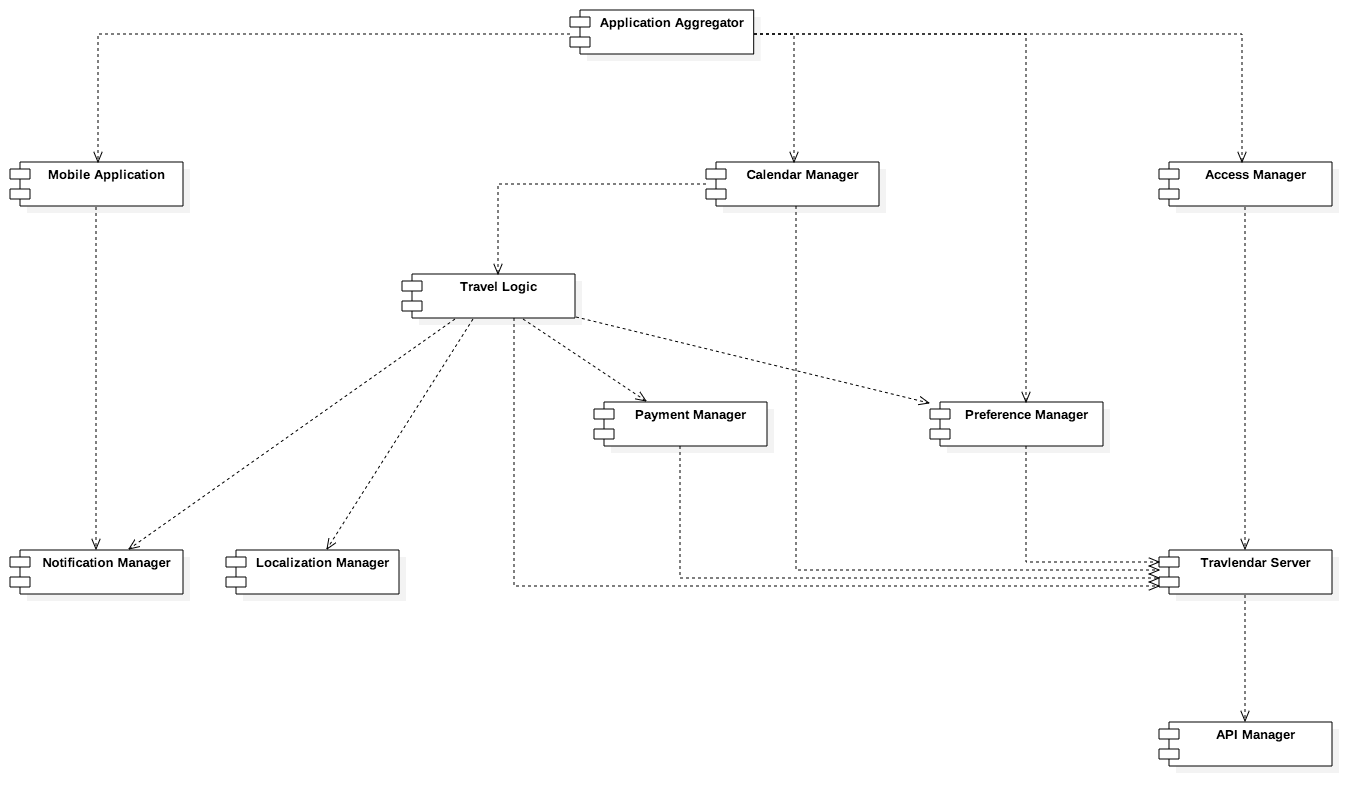
\includegraphics[width=0.9\textwidth]{dependencyTree/dependencyTreeComponent}
		\caption{Dependency tree of components: high level view.}
		\label{DependencyTreehighLevel}
	\end{figure}
	
	\vfill
	
	\begin{figure}[H]
		\centering
		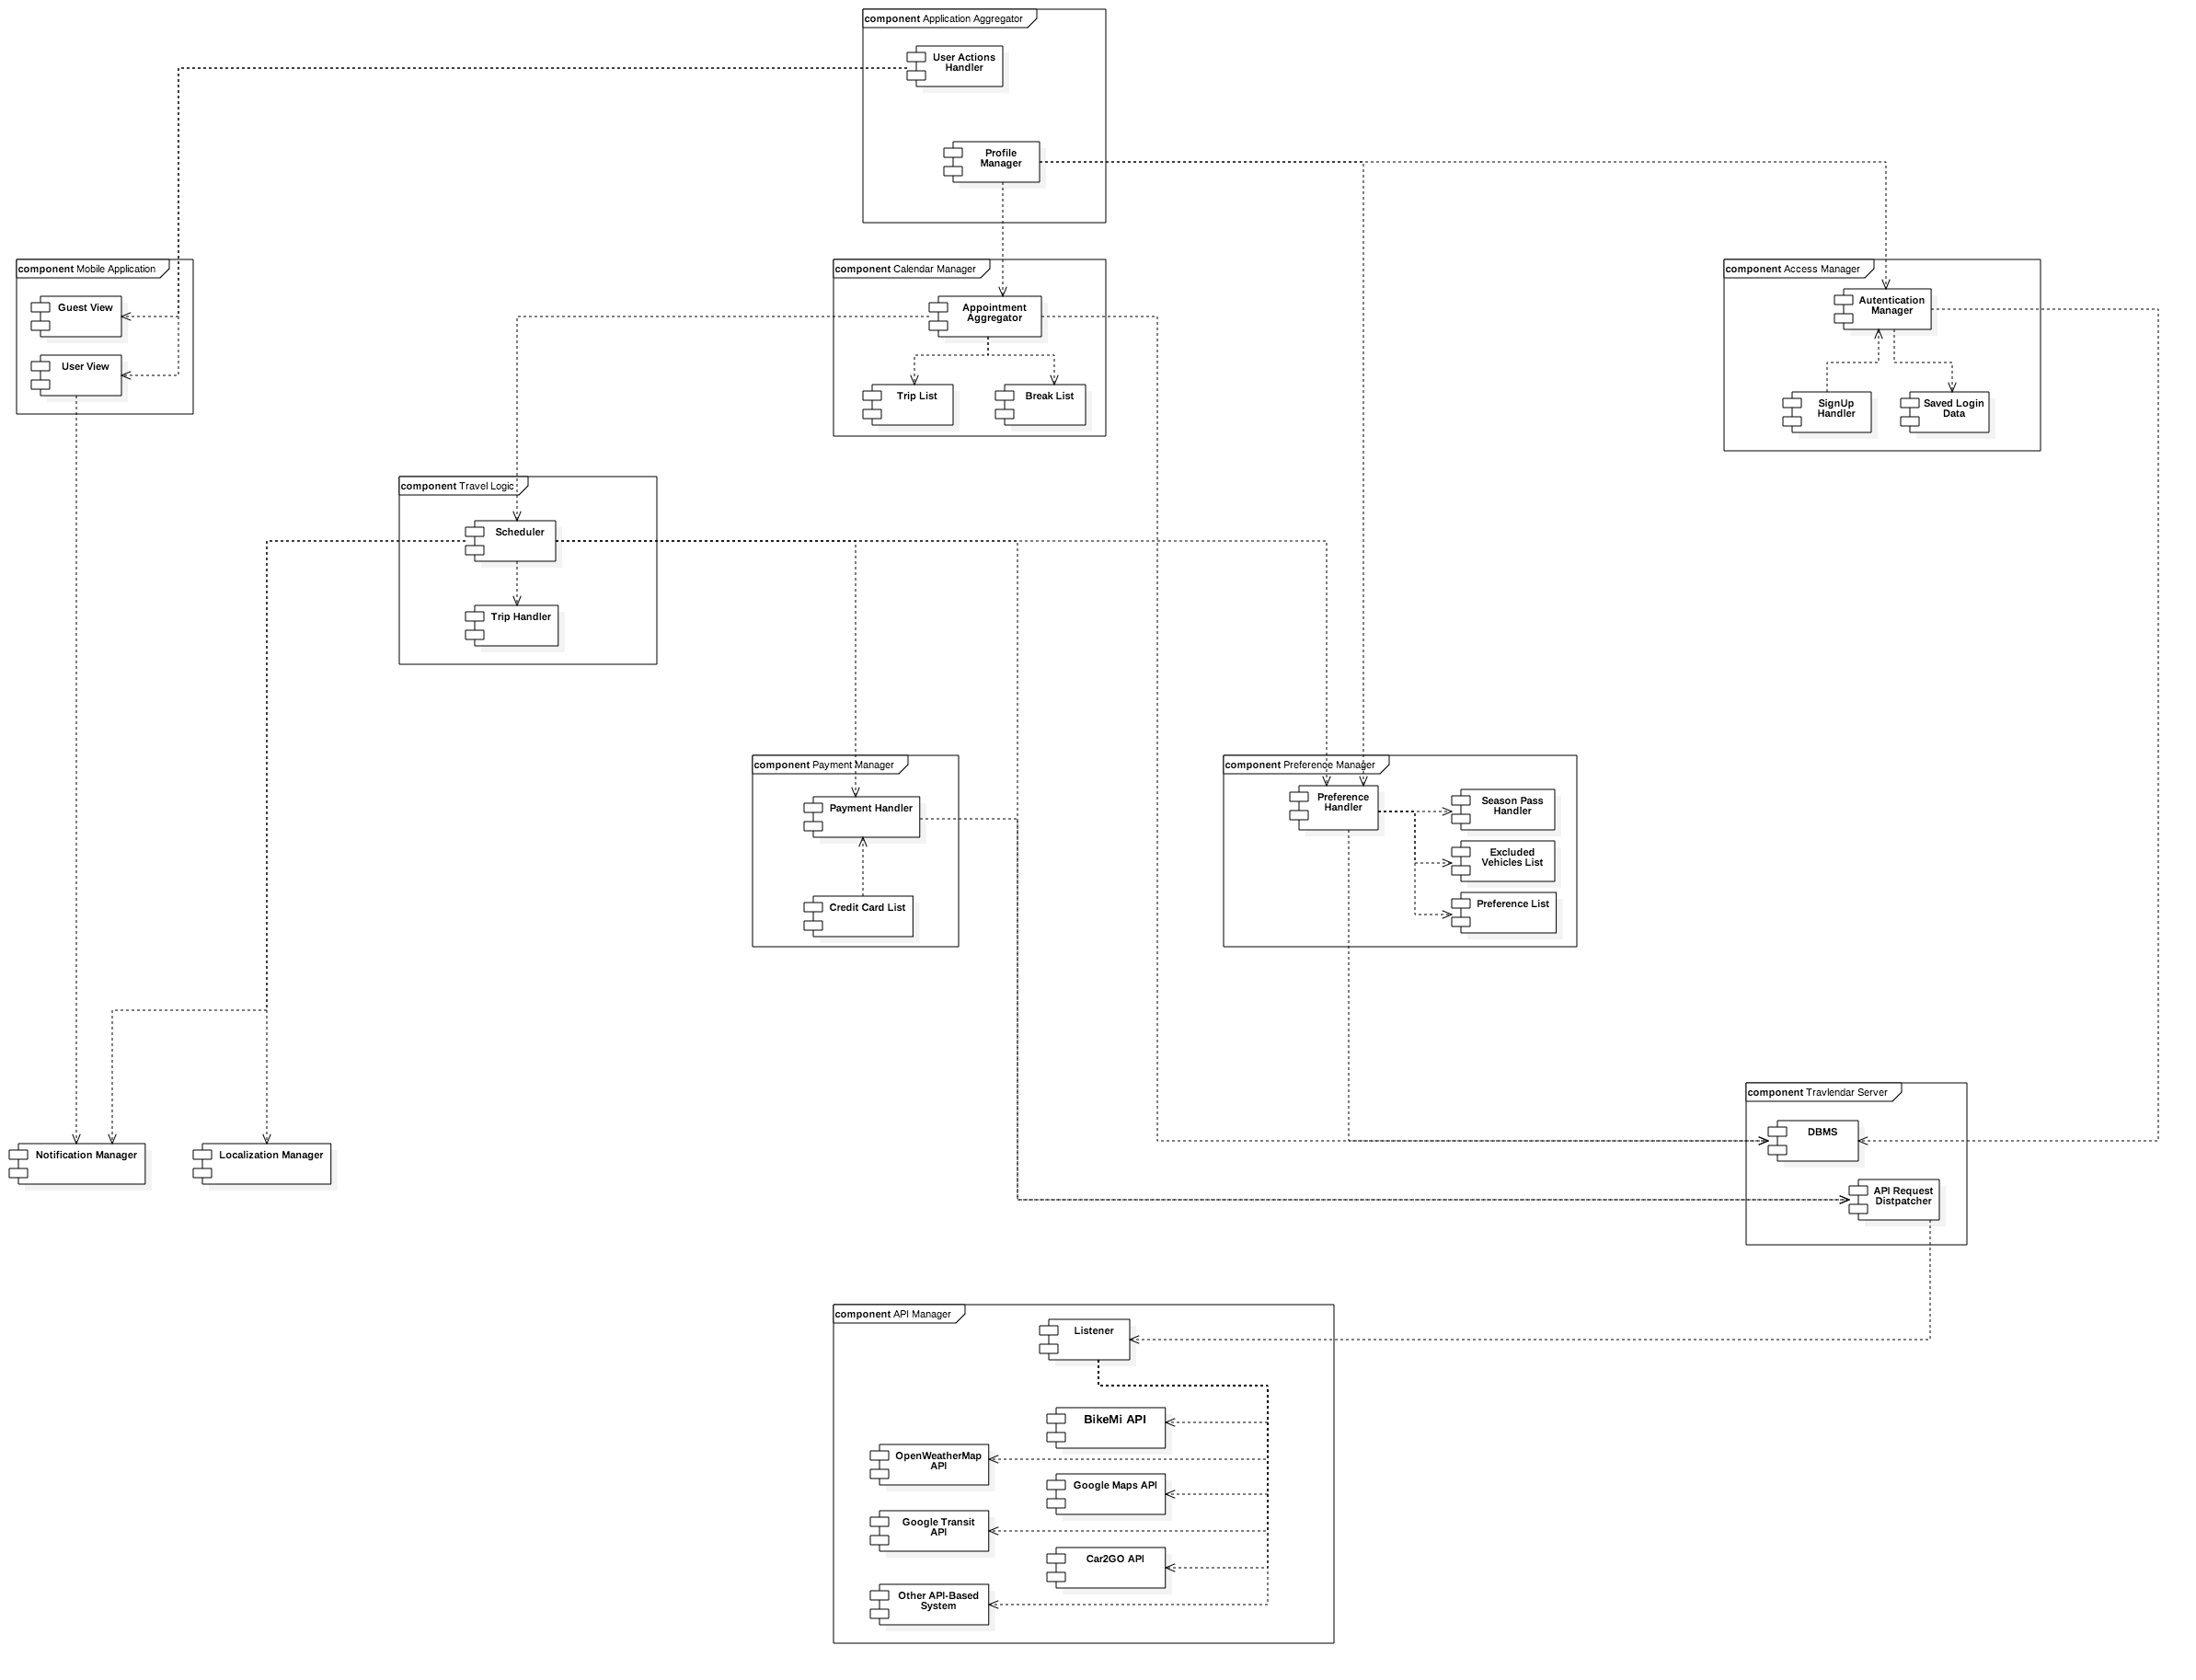
\includegraphics[width=0.9\textwidth]{dependencyTree/dependencyTreeSubcomponents}
		\caption{Dependency tree of components: complete system view.}
		\label{DependencyTreeComplete}
	\end{figure}

\subsubsection{Sequence of component integration}
	From a component perspective we can safely say we adopted a bottom-up policy for the integration plan, while we also used a critical-first approach in sub-components integration (requiring, therefore, stubs in such cases). 
	Our choice has mainly been driven by its ease and by the relatively small scale of our system.
	
	Sequence of component/function integration.
	It's time for us to detail the integration order of our components, delving in what we simply anticipated with our dependency diagrams.
	\begin{description}
	\item[Component]: API Manager.\\
		\textit{Internal integration strategy}: Bottom - Up.\\
		\textit{Integration order}:
		\begin{itemize}
			\item[-] Google Maps API.
			\item[-] OpenWeatherMap.
			\item[-] Google Transit API.
			\item[-] Car2Go API.
			\item[-] BikeMi API.
			\item[-] Other API-Based System.
			\item[-] Listener.
		\end{itemize}
		
		\begin{figure}[H]
			\centering
			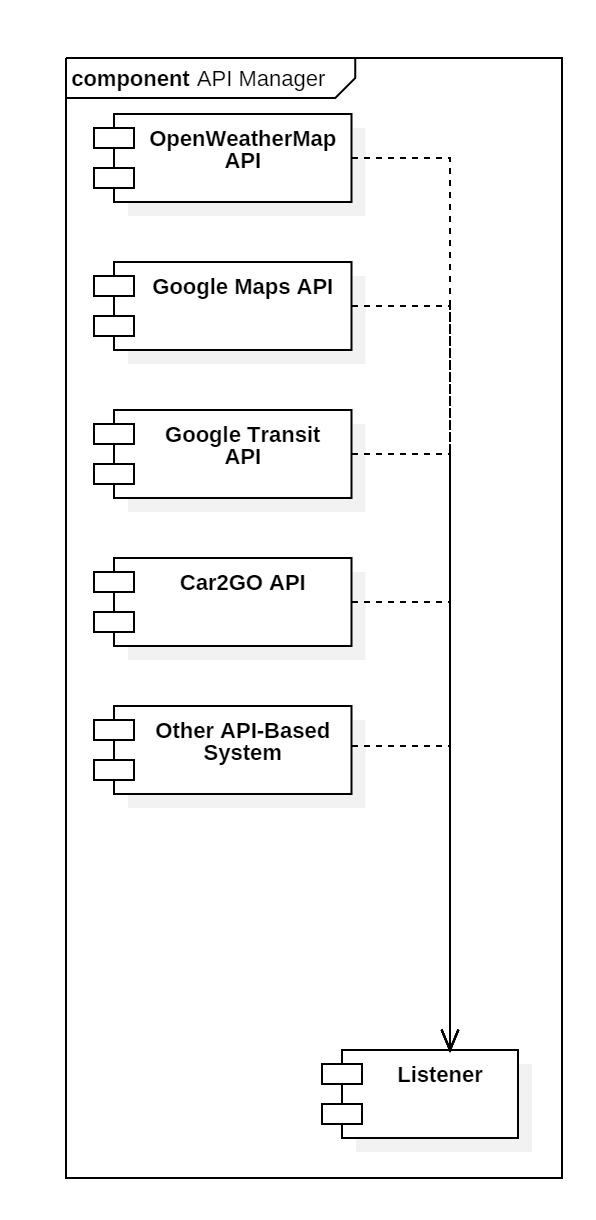
\includegraphics[width=0.5\textwidth]{IntegrationPlan/APIManager}
		\end{figure}
		
		
	\vskip1.5cm
	\item[Component]: Travlendar Server.\\
		\textit{Internal integration strategy}: Critical - First.\\
		\textit{Integration order}:
		\begin{itemize}
			\item[-] DBMS.
			\item[-] API Request Dispatcher.
		\end{itemize}
		
		\begin{figure}[H]
			\centering
			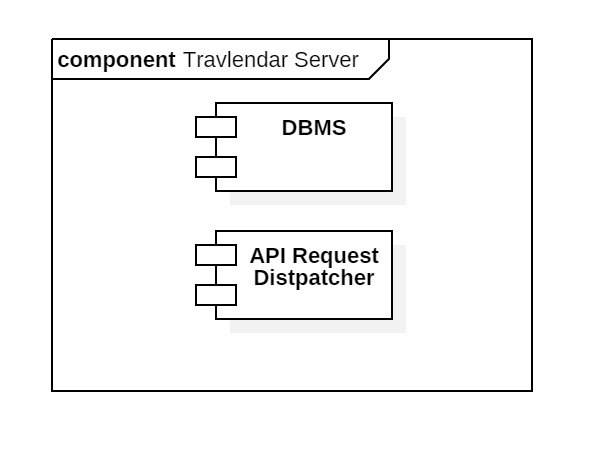
\includegraphics[width=0.5\textwidth]{IntegrationPlan/travlendarServer}
		\end{figure}
	
	
	\vskip1.5cm
	\item[Component]: Localization Manager doesn't need sub-components integration plan.

	\vskip1.5cm
	\item[Component]: Notification Manager doesn't need sub-components integration plan.
	
	\vskip1.5cm
	\item[Component]: Payment Manager.\\
		\textit{Internal integration strategy}: Bottom - Up.\\
		\textit{Integration order}:
		\begin{itemize}
			\item[-] Payment Handler.
			\item[-] Purchase History.
		\end{itemize}
		
		\begin{figure}[H]
			\centering
			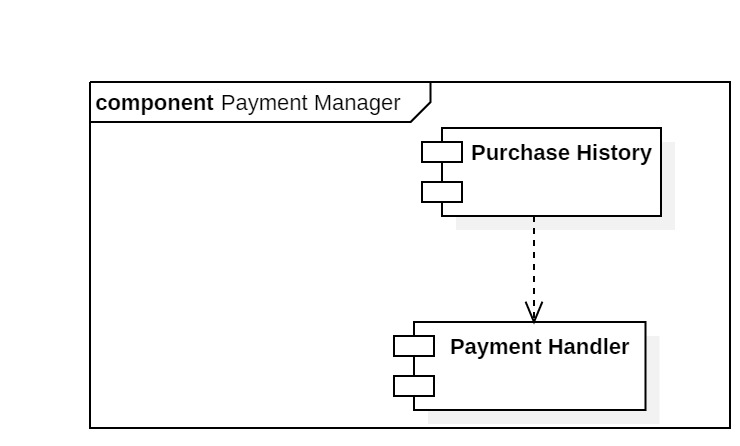
\includegraphics[width=0.5\textwidth]{IntegrationPlan/paymentManager}
		\end{figure}
	
	
	\vskip1.5cm
	\item[Component]: Preference Manager.\\
		\textit{Internal integration strategy}: Bottom - Up\\
		\textit{Integration order}:
		\begin{itemize}
			\item[-] Excluded Vehicles List.
			\item[-] Season Pass Handler.
			\item[-] Preferences List.
			\item[-] Preference Handler.
		\end{itemize}
		
		\begin{figure}[H]
			\centering
			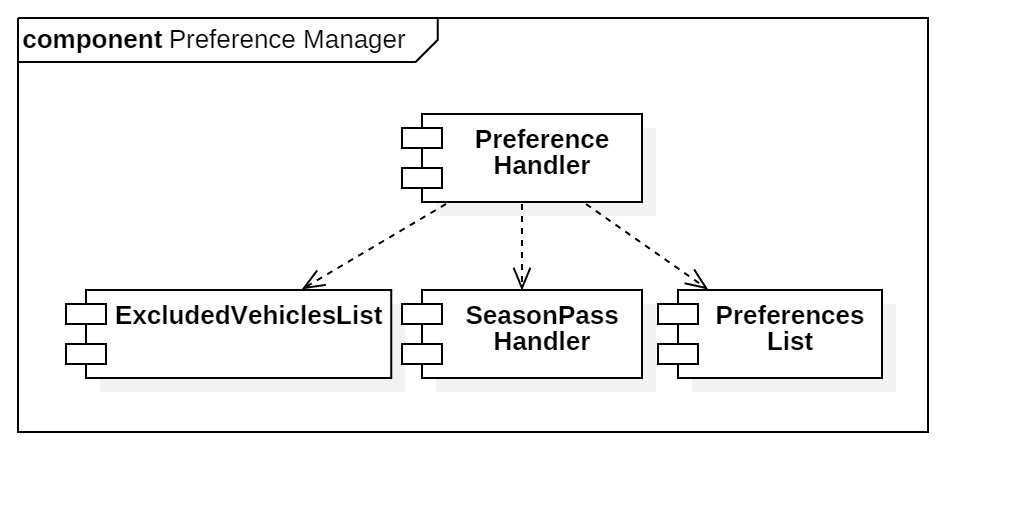
\includegraphics[width=0.5\textwidth]{IntegrationPlan/preferenceManager}
		\end{figure}
		
		
	\vskip1.5cm
	\item[Component]: Travel Logic.\\
		\textit{Internal integration strategy}: Bottom - Up.\\
		\textit{Integration order}:
		\begin{itemize}	
			\item[-] Trip Handler.
			\item[-] Scheduler.
		\end{itemize}
		
		\begin{figure}[H]
			\centering
			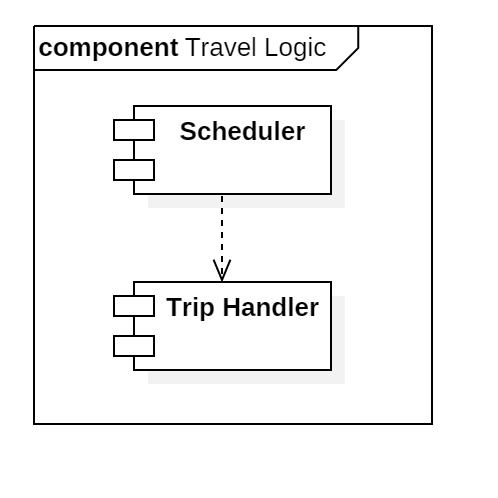
\includegraphics[width=0.5\textwidth]{IntegrationPlan/travelLogic}
		\end{figure}
		
		
	
	\vskip1.5cm
	\item[Component]: Mobile Application.\\
		\textit{Internal integration strategy}: Critical - First.\\
		\textit{Integration order}:
		\begin{itemize}
			\item[-] User View.
			\item[-] Guest View.
		\end{itemize}
		
		\begin{figure}[H]
			\centering
			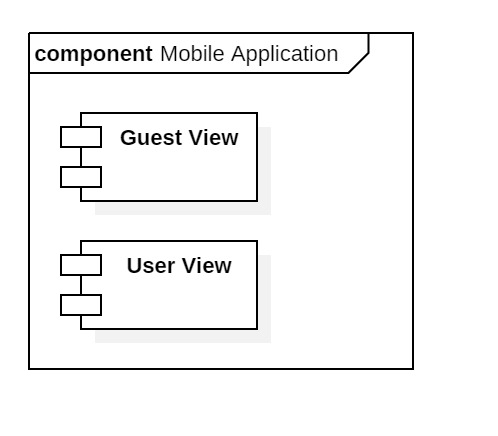
\includegraphics[width=0.5\textwidth]{IntegrationPlan/mobileApplication}
		\end{figure}
	
	
	
	\vskip1.5cm
	\item[Component]: Calendar Manager.\\
		\textit{Internal integration strategy}: Bottom - Up.\\
		\textit{Integration order}:
		\begin{itemize}
			\item[-] Trip List.
			\item[-] Break List.
			\item[-] Appointment Aggregator.
		\end{itemize}
		
		\begin{figure}[H]
			\centering
			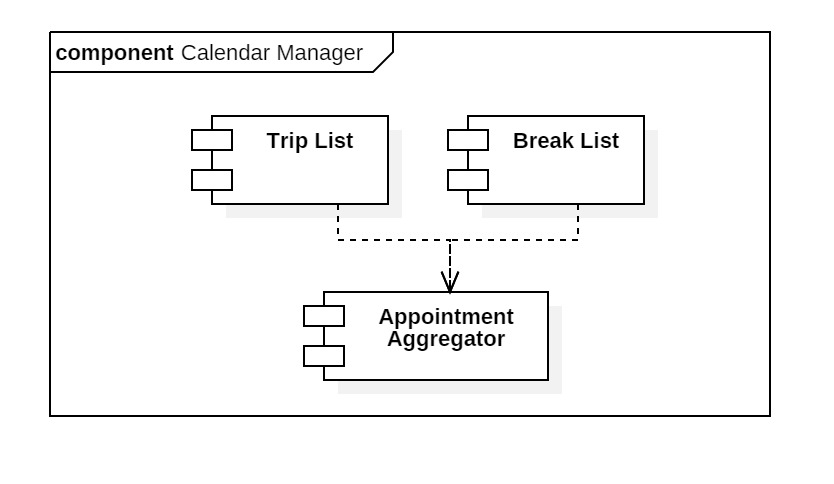
\includegraphics[width=0.5\textwidth]{IntegrationPlan/calendarManager}
		\end{figure}


	\vskip1.5cm
	\item[Component]: Access Manager.\\
		\textit{Internal integration strategy}: Critical - first.\\
		\textit{Integration order}:
		\begin{itemize}
			\item[-] Authentication Manager.
			\item[-] SignUp Handler.
			\item[-] Saved Login Data.
		\end{itemize}
		
		\begin{figure}[H]
			\centering
			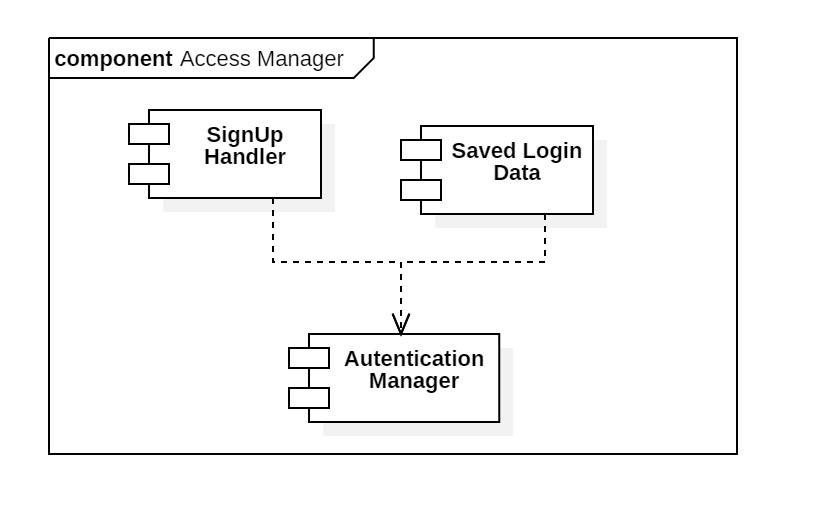
\includegraphics[width=0.5\textwidth]{IntegrationPlan/accessManager}
		\end{figure}
		
		
	\vskip1.5cm
	\item[Component]: Application Aggregator.\\
		\textit{Internal integration strategy}: Critical-First.\\
		\textit{Integration order}:
		\begin{itemize}
			\item[-] Profile Manager.
			\item[-] User Actions Handler.
		\end{itemize}
		
		\begin{figure}[H]
			\centering
			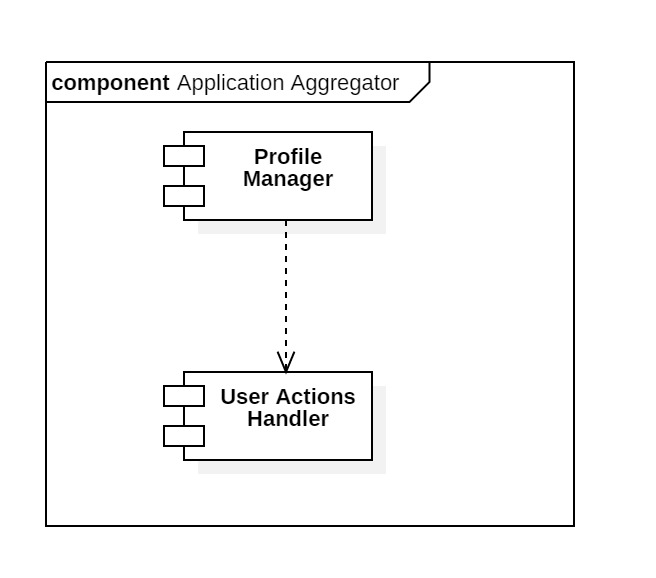
\includegraphics[width=0.5\textwidth]{IntegrationPlan/applicationAggregator}
		\end{figure}
		
\end{description}
	

\vfill
\subsubsection{Subsystem integration sequence}
	The integration of the macro-components is performed, as said, in a bottom-up fashion. Below are the 6 steps in which this process has been divided for scheduling reasons.
	Inside a single step, multiple macro-components participate in the integration, each one relying on the macro-components in the previous levels.
	
	\begin{description}
	
	\item Step 1		
		\begin{figure}[H]
			\centering
			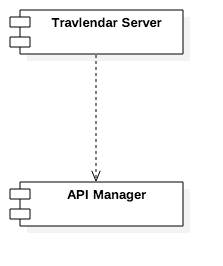
\includegraphics[width=0.25\textwidth]{componentIntegrationStepByStep/step1}
			\caption{Subsystem integration sequence: step 1.}
		\end{figure}
	
	\vfill
	\item Step 2
		\begin{figure}[H]
			\centering
			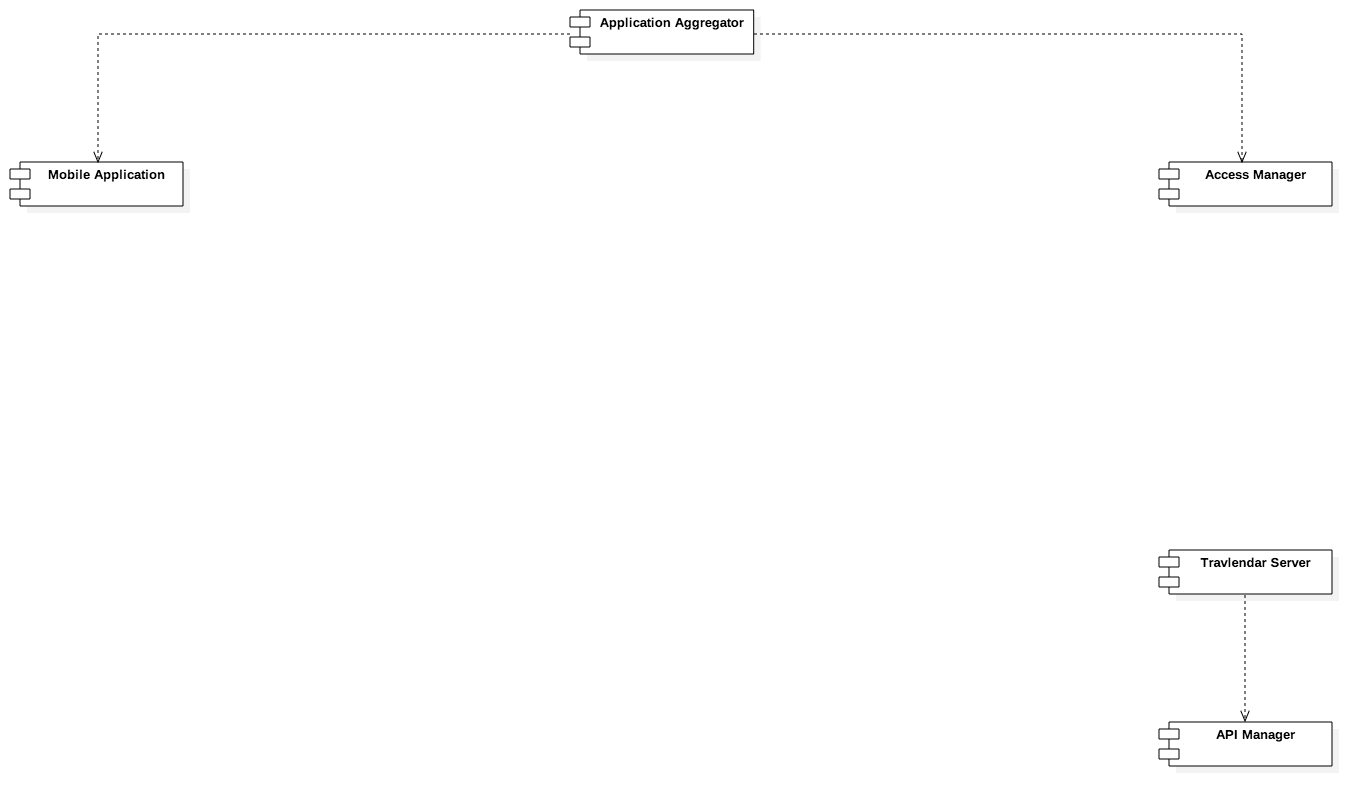
\includegraphics[width=0.95\textwidth]{componentIntegrationStepByStep/step2}
			\caption{Subsystem integration sequence: step 2.}
		\end{figure}
	
	\bigskip
	\item Step 3
		\begin{figure}[H]
			\centering
			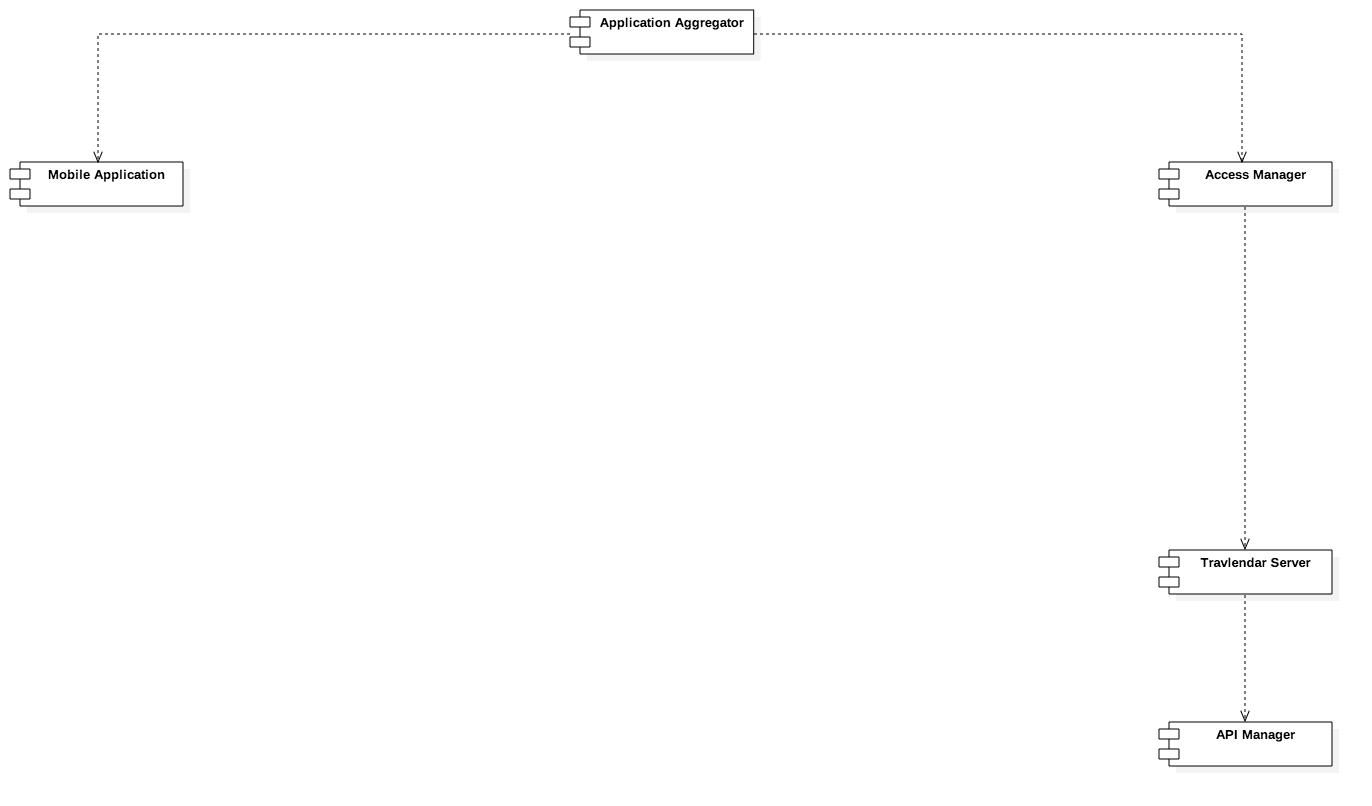
\includegraphics[width=0.95\textwidth]{componentIntegrationStepByStep/step3}
			\caption{Subsystem integration sequence: step 3.}
		\end{figure}
		
	\bigskip
	\item Step 4
		\begin{figure}[H]
			\centering
			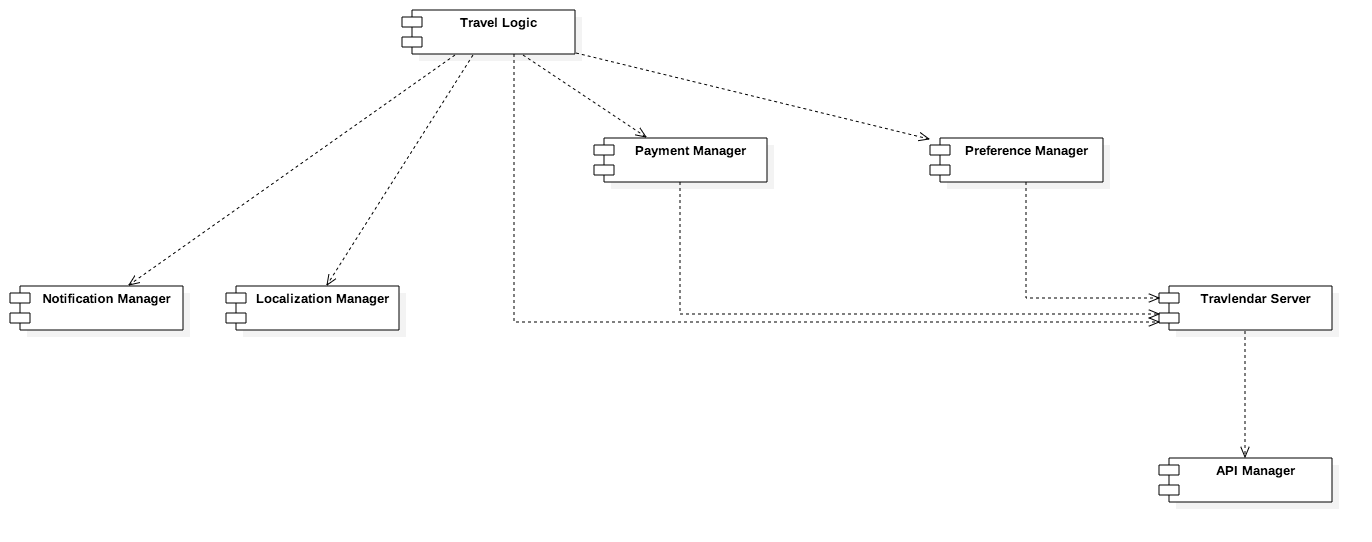
\includegraphics[width=0.95\textwidth]{componentIntegrationStepByStep/step4}
			\caption{Subsystem integration sequence: step 4.}
		\end{figure}
		
	\bigskip
	\item Step 5
		\begin{figure}[H]
			\centering
			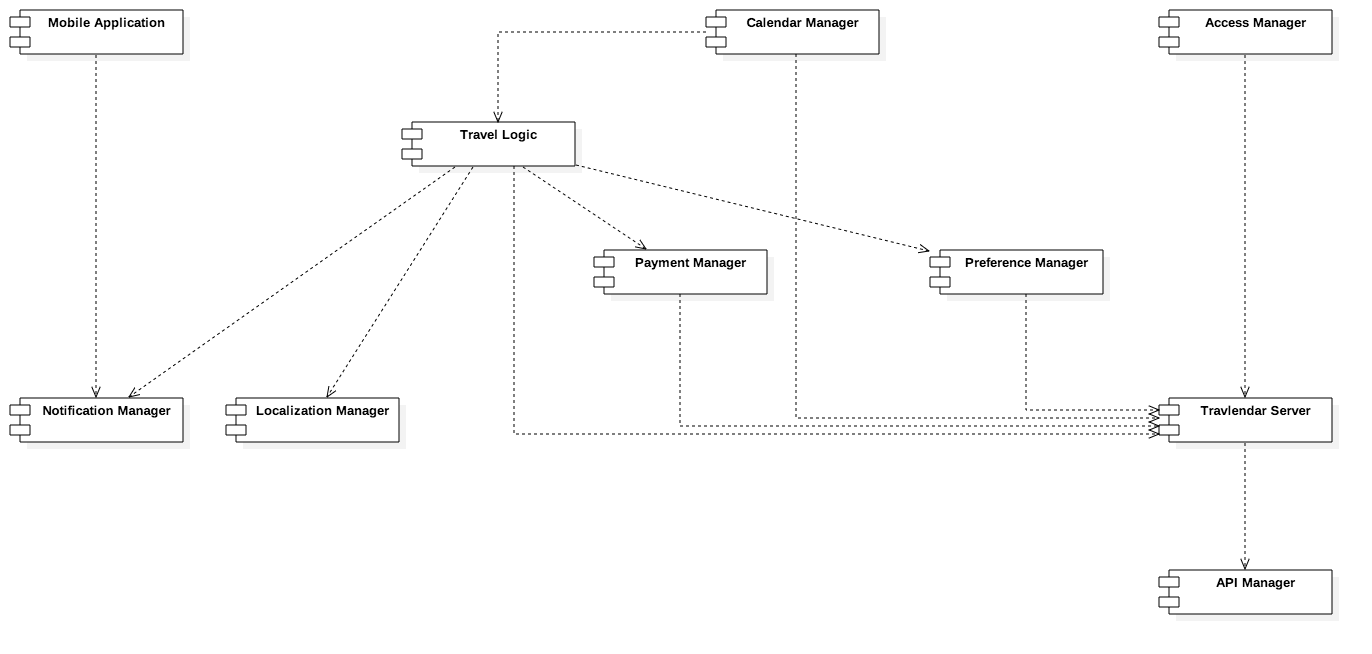
\includegraphics[width=0.95\textwidth]{componentIntegrationStepByStep/step5}
			\caption{Subsystem integration sequence: step 5.}
		\end{figure}
		
	\bigskip	
	\item Step 6
		\begin{figure}[H]
			\centering
			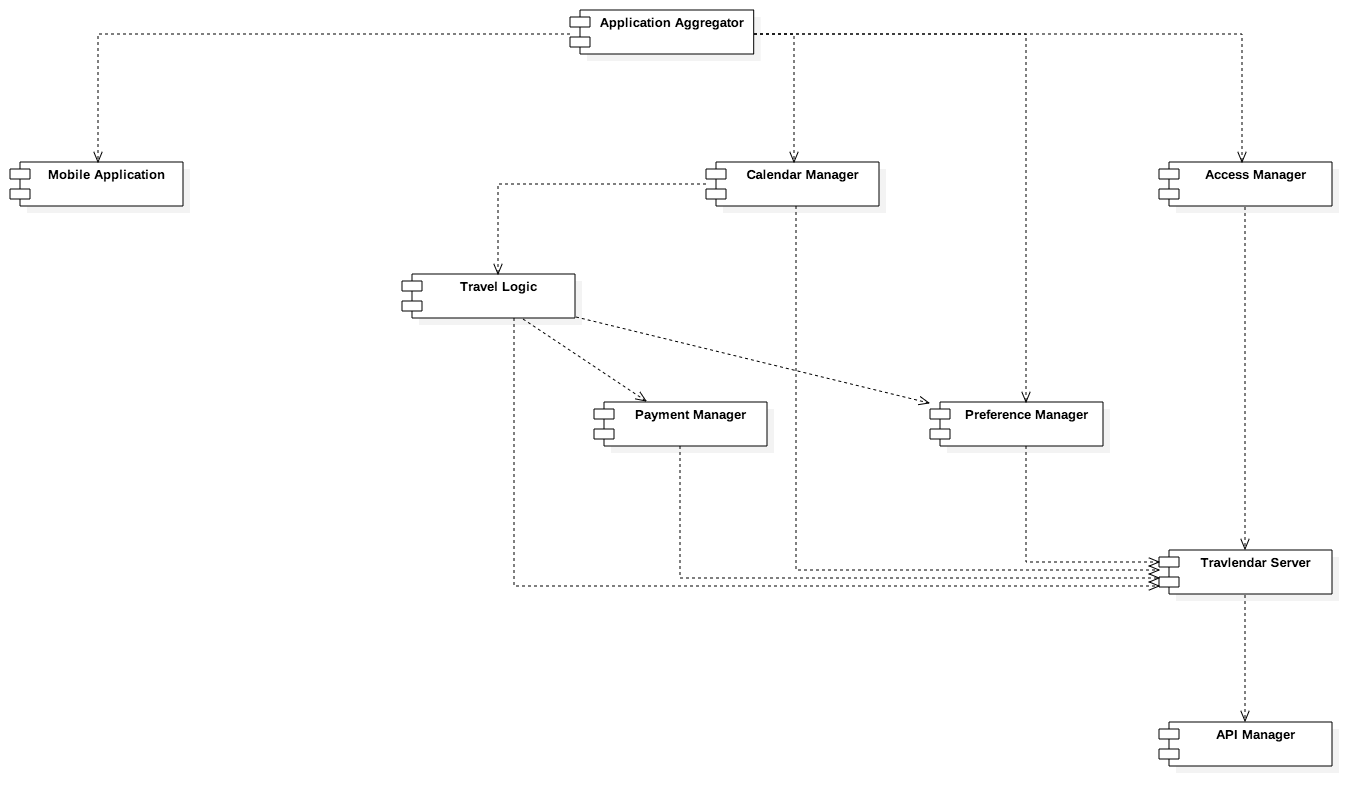
\includegraphics[width=0.95\textwidth]{componentIntegrationStepByStep/step6}
			\caption{Subsystem integration sequence: step 6.}
		\end{figure}

	\end{description}
	

			
		\subsection{Individual Steps and Test Description}
			The components will be tested following the interfaces they share and that we previously described, testing core methods also in case of sub-components integration.
Our main goal is to spot any kind of faults and failures, focusing in particular on input domains, covering the restricted spectrum of system reactions.
Because of this, we'll detail the tests in easy-to-consult tables, each introduced by the components and subcomponents that are required.
Each table represents an interface method, and on two columns we'll detail each input and its expected result.
We'll follow a bottom-up approach that requires the creation of drivers from time to time.

\subsubsection{API Communication Service}
	
	\textbf{OpenWeatherMap API,Listener}\\
		\begin{tabular}{| p{0.3\textwidth} |p{0.6\textwidth}|}
			\hline
			\hline
			
			\multicolumn{2}{|c|} {getWeatherInfo() }\\
			\hline
			
			\textbf{Input} & \textbf{Effect}.\\
			\hline
			\hline
			
			NullArgument.		&		NullArgumentException is raised.\\
			\hline
			
			Invalid Location	.	&		OpenWeather services return the information cannot be retrieved and the Listener signals the location is wrong.\\
			\hline		
			
			Valid Location.		&		Listener retrieves the required data structure from OpenWeatherMap and formats it.\\
			\hline
			\hline
		\end{tabular}
	
	\vskip1cm
	
	\noindent	
	\textbf{GoogleMapsAPI, Listener}\\
		\begin{tabular}{| p{0.3\textwidth} |p{0.6\textwidth}|}
			\hline
			\hline
			
			\multicolumn{2}{|c|} {getTravelTime() }\\
			\hline
			
			\textbf{Input}.		&		\textbf{Effect}.\\
			\hline
			\hline
			
			NullArgument.	&		NullArgumentException is raised.\\
			\hline
			
			Invalid Start Location/Destination Location.		&		GMAPS APIs signals one (or both) the locations are wrong and the Listener echoes this back.\\
			\hline		
			
			Valid Start Location and Destination Location.	&	 Listener retrieves the required data structure from GMAPS API.\\
			\hline
			\hline
		\end{tabular}

	\vskip1cm

	\noindent
	\textbf{Car2Go API, Listener}\\
	\textbf{BikeMi, Listener}\\
	\textbf{ Other API-Based Systems, Listener}\\
		\begin{tabular}{| p{0.3\textwidth} |p{0.6\textwidth}|}
			\hline
			\hline
			
			\multicolumn{2}{|c|} {findNearestVehicle() }\\
			\hline
	
			\textbf{Input}.		&		\textbf{Effect}.\\
			\hline
			\hline

			NullArgument.	&		NullArgumentException is raised.\\
			\hline
	
			Invalid Location or Location out of the boundaries.		&		The external signals the location is out of its service boundaries.\\
			\hline		
		
			Valid Location.		&		Listener retrieves the required data structure from the external API and formats it in order for it to be navigable within the mobile application.\\
			\hline
			\hline
		\end{tabular}

	\vskip1cm

	\noindent
	\textbf{Car2Go API, Listener}\\
	\textbf{BikeMi, Listener}\\
	\textbf{Other API-Based Systems, Listener}\\
		\begin{tabular}{| p{0.3\textwidth} |p{0.6\textwidth}|}
			\hline
			\hline
			
			\multicolumn{2}{|c|} {getReservationConfirmation() }\\
			\hline
			
			\textbf{Input}.		&		\textbf{Effect}.\\
			\hline
			\hline
			
			NullArgument.		&		NullArgumentException is raised.\\
			\hline
			
			Invalid Reservation Code.		&		The external service can’t provide reservation data, and it sends only a message error, that Listener echoes back.\\
			\hline
			
			Valid Reservation Code.	&		Listener retrieves the required data structure from the external API and formats it in order for it to be navigable within the mobile application.\\
			\hline
			\hline
		\end{tabular}

	\vskip1cm

	\noindent
	\textbf{Google Transit API, Listener}\\
		\begin{tabular}{| p{0.3\textwidth} |p{0.6\textwidth}|}
			\hline
			\hline
			
			\multicolumn{2}{|c|} {getTrafficInfo() }\\
			\hline
			
			\textbf{Input}.		&		\textbf{Effect}.\\
			\hline
			\hline
	
			NullArgument.	&		NullArgumentException is raised.\\
			\hline

			Invalid Path.		&		GMAPS APIs can’t find the route and send back a message to document the impossibility of monitoring the traffic. Listener echoes this back.\\
			\hline

			Valid Path & Google Transit API provides the required information about traffic and Listener sends them back.\\
			\hline
			\hline
		\end{tabular}

	\vskip1cm

	\noindent
	\textbf{Listener, API Request Dispatcher}\\
	\begin{flushleft} %two tables are alligned to the left

		\begin{tabular}{| p{0.3\textwidth} |p{0.6\textwidth}|}
			\hline
			\hline
			
			\multicolumn{2}{|c|} {provideMap() }\\
			\hline

			\textbf{Input}.		&		\textbf{Effect}.\\
			\hline
			\hline

			NullArgument.		&		NullArgumentException is raised.\\
			\hline

			Start Location and End Location.		&		Path from Start Location until End Location is raised.\\
			\hline

			Location and Firm’s name.			&		Path from Location until nearest vehicle is raised.\\
			\hline

			Location and Day.		&		Weather information is shown.\\
			\hline
			\hline
		\end{tabular}	
		\\
		\vskip0.25cm		
		\begin{tabular}{| p{0.3\textwidth} |p{0.6\textwidth}|}
			\hline
			\hline
			
			\multicolumn{2}{|c|} {retrievePaymentInfo() }\\
			\hline
			
			\textbf{Input}.		&		\textbf{Effect}.\\
			\hline
			\hline
			
			NullArgument.		&		NullArgumentException is raised.\\
			\hline
			
			Valid parameters.		&		A request of payment is sent.\\
			\hline
			
			Invalid parametert.		&		InvalidArgumentException is raised.\\
			\hline
			\hline
		\end{tabular}
	\end{flushleft}				


\vfill		
\subsubsection{Travlendar Server}
	\textbf{API Request Dispatcher, Payment Handler}\\
		\begin{tabular}{| p{0.3\textwidth} |p{0.6\textwidth}|}
		\hline
		\hline
		
		\multicolumn{2}{|c|} {APIRequest() }\\
		\hline
		
		\textbf{Input}.		&		\textbf{Effect}.\\
		\hline
		\hline
		
		NullArgument.		&		NullArgumentException is raised.\\
		\hline
		
		Valid Argument.		&		A payment request is sent to the Server.\\
		\hline
		
		Invalid Argument.		&		InvalidArgumentException is raised.\\
		\hline
	\end{tabular}

	\vskip1cm

	\noindent
	\textbf{API Request Dispatcher, Scheduler}\\
		\begin{tabular}{| p{0.3\textwidth} |p{0.6\textwidth}|}
			\hline
			\hline

			\multicolumn{2}{|c|} {APIRequest() }\\
			\hline

			\textbf{Input}.		&		\textbf{Effect}.\\
			\hline
			\hline
			
			NullArgument.		&		NullArgumentException is raised.\\
			\hline
		
			Valid Combination of Location, Data and Vehicle’s Firm is allowed.		&		A request is sent to the respective dispatcher.\\
			\hline
			
			Invalid Argument.		&		InvalidArgumentException is raised.\\
			\hline
		\end{tabular}

	\vskip1cm

	\noindent
	\textbf{DBMS, Authentication Manager}\\
		\begin{tabular}{| p{0.3\textwidth} |p{0.6\textwidth}|}
			\hline
			\hline
	
			\multicolumn{2}{|c|} {requestUserCalendar() }\\
			\hline

			\textbf{Input}.		&		\textbf{Effect}.\\
			\hline
			\hline

			NullArgument.		&		NullArgumentException is raised.\\
			\hline
		
			Invalid Argument.		&		InvalidArgumentException is raised.\\
			\hline
	
			User Credentials.		&		An access request is sent to DBMS.\\
			\hline
			\hline
		\end{tabular}

	\vskip1cm

	\noindent
	\textbf{DBMS, Autentication Manager}\\
		\begin{tabular}{| p{0.3\textwidth} |p{0.6\textwidth}|}
			\hline
			\hline
			
			\multicolumn{2}{|c|} {requestUserPreferences() }\\
			\hline
			
			\textbf{Input}.		&		\textbf{Effect}.\\
			\hline
			\hline
		
			NullArgument.		&		NullArgumentException is raised.\\
			\hline
		
			Invalid Argument.		&		InvalidArgumentException is raised.\\
			\hline
			
			User Credentials.		&		An access request of user preferences is sent to DBMS.\\
			\hline
			\hline
		\end{tabular}

	\vskip1cm

	\noindent
	\textbf{DBMS, Autentication Manager}\\
		\begin{tabular}{| p{0.3\textwidth} |p{0.6\textwidth}|}
			\hline
			\hline
		
			\multicolumn{2}{|c|} {updateUserCalendar() }\\
			\hline
			
			\textbf{Input}.		&		\textbf{Effect}.\\
			\hline
			\hline
		
			NullArgument.		&		NullArgumentException is raised.\\
			\hline
	
			Invalid Argument.		&		InvalidArgumentException is raised.\\
			\hline
		
			User Credentials and New DataCalendar.		&		User Calendar is update.\\
			\hline
			\hline
		\end{tabular}
		
	\vskip1cm

	\noindent
	\textbf{DBMS, Autentication Manager}\\
		\begin{tabular}{| p{0.3\textwidth} |p{0.6\textwidth}|}
			\hline
			\hline
		
			\multicolumn{2}{|c|} {updateUserPreferences() }\\
			\hline
			
			\textbf{Input}.		&		\textbf{Effect}.\\
			\hline
			\hline
		
			NullArgument.		&		NullArgumentException is raised.\\
			\hline

			Invalid Argument.		&		InvalidArgumentException is raised.\\
			\hline

			User Credentials and New DataPreferences.		&		User Preferences is update.\\
			\hline
			\hline
		\end{tabular}

	\vskip1cm

	\noindent
	\textbf{DBMS, Autentication Manager}\\
		\begin{tabular}{| p{0.3\textwidth} |p{0.6\textwidth}|}
			\hline
			\hline
			
			\multicolumn{2}{|c|} {registerUser() }\\
			\hline
			
			\textbf{Input}.		&		\textbf{Effect}.\\
			\hline
			\hline

			NullArgument.		&		NullArgumentException is raised.\\
			\hline

			Invalid Argument.		&		InvalidArgumentException is raised.\\
			\hline

			Valid Combination of User Credential and User Information.		&		New User Profile is created.\\
			\hline
			\hline
		\end{tabular}

	\vskip1cm

	\noindent
	\textbf{DBMS, Autentication Manager}\\
		\begin{tabular}{| p{0.3\textwidth} |p{0.6\textwidth}|}
			\hline
			\hline
		
			\multicolumn{2}{|c|} {checkCredentialUser() }\\
			\hline
		
			\textbf{Input}.		&		\textbf{Effect}.\\
			\hline
			\hline

			NullArgument.		&		NullArgumentException is raised.\\
			\hline

			Invalid Argument.		 &			False.\\
			\hline	
	
			User Credentials insert		&		True.\\
			\hline		
			\hline
		\end{tabular}
		
		
\vfill
\subsubsection{Payment Manager}
	
	\textbf{Payment Handler, Purchase History}\\
		\begin{tabular}{| p{0.3\textwidth} |p{0.6\textwidth}|}
			\hline
			\hline
			
			\multicolumn{2}{|c|} {addPaymentMethod() }\\
			\hline
			
			\textbf{Input}.		&		\textbf{Effect}.\\
			\hline
			\hline
			
			NullArgument.		&		NullArgumentException is raised.\\
			\hline
			
			Credit Card Data and linked Transaction information.		&		Data is stored in Purchase History.\\
			\hline
			
			Invalid Data.		&		Nothing changes and the input is rejected.\\
			\hline
			\hline
		\end{tabular}

	\vskip1cm

	\noindent
	\textbf{Payment Handler, Purchase History}\\
		\begin{tabular}{| p{0.3\textwidth} |p{0.6\textwidth}|}
			\hline
			\hline
			
			\multicolumn{2}{|c|} {deletePaymentMethod() }\\
			\hline
			
			\textbf{Input}.		&		\textbf{Effect}.\\
			\hline
			\hline

			NullArgument.		&		NullArgumentException is raised.\\
			\hline
			
			Credit Card Data.		&		Credit Card Data and the linked transactions stored in Purchase History are deleted.\\
			\hline
			
			Invalid Input.		&		Everything is unchanged in Purchase History.\\
			\hline
			\hline
		\end{tabular}

	\vskip1cm

	\noindent
	\textbf{Payment Handler, Purchase History}\\
		\begin{tabular}{| p{0.3\textwidth} |p{0.6\textwidth}|}
			\hline
			\hline
			
			\multicolumn{2}{|c|} {showPaymentRecord() }\\
			\hline
			
			\textbf{Input}.		&		\textbf{Effect}.\\
			\hline
			\hline
	
			NullArgument.		&		The payment record is returned in the correct data structure.\\
			\hline
			
			Any Parameter.		&		InvalidArgumentException is raised.\\
			\hline
			
			Invalid Input.		&		InvalidArgumentException is thrown and everything is unchanged in Purchase History.\\
			\hline
			\hline
		\end{tabular}
	
	\vskip1cm

	\noindent
	\textbf{Payment Handler, Scheduler}\\
		\begin{tabular}{| p{0.3\textwidth} |p{0.6\textwidth}|}
			\hline
			\hline
			
			\multicolumn{2}{|c|} {addPayment() }\\
			\hline
			
			\textbf{Input}.		&		\textbf{Effect}.\\
			\hline
			
			NullArgument.		&		NullArgumentException is raised.\\
			\hline
			
			Valid Ticket.		&		A payment request is shown.\\
			\hline 
			
			Invalid Input.		&		invalidArgumentException is thrown and everything is unchanged in Purchase History.\\
			\hline
			\hline
		\end{tabular}


\vfill
\subsubsection{Preference Manager}

	\textbf{Preference Handler, Excluded Vehicle List}\\
		\begin{tabular}{| p{0.3\textwidth} |p{0.6\textwidth}|}
			\hline
			\hline
			
			\multicolumn{2}{|c|} {setExcludedVehicles() }\\
			\hline
			
			\textbf{Input}.		&		\textbf{Effect}.\\
			\hline
			\hline
			
			NullArgument.		&		NullArgumentException is thrown.\\
			\hline
			
			Argument not corresponding to a collection of vehicle objects.		&		InvalidArgumentException is thrown.\\
			\hline

			Valid collection of vehicle objects.		&		The list of excluded vehicles is updated to become as the input.\\
			\hline
			\hline
		\end{tabular}

	\vskip1cm

	\noindent
	\textbf{Preference Handler, SeasonPass Handler}\\
		\begin{tabular}{| p{0.3\textwidth} |p{0.6\textwidth}|}
			\hline
			\hline
			
			\multicolumn{2}{|c|} {setSeasonPass() }\\
			\hline
			
			\textbf{Input}.		&		\textbf{Effect}.\\
			\hline
			\hline
			
			NullArgument.		&		NullArgumentException is thrown.\\
			\hline
			
			Argument not corresponding to a collection of seasonPasses.		&		InvalidArgumentException is thrown.\\
			\hline
			
			Valid collection of seasonPasses.		&		The list of seasonPasses is updated to become the same as the input.\\
			\hline
			\hline
		\end{tabular}

	\vskip1cm

	\noindent
	\textbf{Preference Handler, Preferences List}\\
	\begin{flushleft}

		\begin{tabular}{| p{0.3\textwidth} |p{0.6\textwidth}|}
			\hline
			\hline
			
			\multicolumn{2}{|c|} {setVehicleTimeSpan() }\\
			\hline
			
			\textbf{Input}.		&		\textbf{Effect}.\\
			\hline
			\hline
			
			NullArgument.		&		NullArgumentException is thrown.\\
			\hline
			
			Argument is not a collection of pairs of vehicles and time spans.		&		InvalidArgumentException is thrown.\\
			\hline

			Argument is a valid collection of pairs of vehicles and time spans.		&		The list of pairs of vehicles and time spans is updated to become the same as the input.\\
			\hline
			\hline
		\end{tabular}		
		\\
		\vskip0.25cm
		\begin{tabular}{| p{0.3\textwidth} |p{0.6\textwidth}|}
			\hline
			\hline
			
			\multicolumn{2}{|c|} {setCarbonFootprints() }\\
			\hline
			
			\textbf{Input}.		&		\textbf{Effect}.\\
			\hline
			\hline
			
			NullArgument.		&		Carbon footprints are not set.\\
			\hline
			
			Invalid non-integer argument.		&		InvalidArgumentException is thrown.\\
			\hline
			
			Valid integer input.		&		Carbon footprints are set as the input commands.\\
			\hline
			\hline
		\end{tabular}
		\\
		\vskip0.25cm
		\begin{tabular}{| p{0.3\textwidth} |p{0.6\textwidth}|}
			\hline
			\hline
			
			\multicolumn{2}{|c|} {setMaxDistancePerVehicle() }\\
			\hline
			
			\textbf{Input}.		&		\textbf{Effect}.\\
			\hline
			\hline
			
			NullArgument.		&		NullArgumentException is thrown.\\
			\hline
			
			Argument is not a collection of pairs of vehicles and integers.		&		InvalidArgumentException is raised.\\
			\hline

			Argument is a valid collection of pairs of vehicles and integers.		&		For each specified vehicle it is set the maximum allowed distance that it can travel.\\
			\hline
			\hline
		\end{tabular}
	
	\end{flushleft}

	\vskip1cm

	\noindent
	\textbf{PreferenceHandler, Scheduler}\\
		\begin{tabular}{| p{0.3\textwidth} |p{0.6\textwidth}|}
			\hline
			\hline
			
			\multicolumn{2}{|c|} {applyConstraints() }\\
			\hline
			
			\textbf{Input}.		&		\textbf{Effect}.\\
			\hline
			\hline
			
			NullArgument.		&		NullArgumentException is thrown.\\
			\hline
			
			Invalid Argoument.		&		InvalidArgumentException is thrown.\\
			\hline
			
			Valide combination of User Credentials and Type of constraint.		&		The list of trips is filtered according to existing preferences.\\
			\hline
			\hline
		\end{tabular}
	
	
\vfill
\subsubsection{Travel Logic}

	\textbf{Scheduler, Trip Handler}\\
		\begin{tabular}{| p{0.3\textwidth} |p{0.6\textwidth}|}
			\hline
			\hline
			
			\multicolumn{2}{|c|} {scheduleEvent() }\\
			\hline
			
			\textbf{Input}.		&		\textbf{Effect}.\\
			\hline
			\hline
			
			NullArgument.		&		NullArgumentException is thrown.\\
			\hline
			
			Argument is not a valid event paired with a location and a date.		&		InvalidArgumentException is thrown.\\
			\hline
		
			Argument is a valid event paired with a location and a date.		&		The event is added and scheduled by the logic of the mobile application.\\
			\hline
			\hline
		\end{tabular}

	\vskip1cm

	\noindent
	\textbf{Scheduler, Appointment Aggregator}\\
	\begin{flushleft}
		\begin{tabular}{| p{0.3\textwidth} |p{0.6\textwidth}|}
			\hline
			\hline
			
			\multicolumn{2}{|c|} {checkIntegrity() }\\
			\hline
			
			\textbf{Input}.		&		\textbf{Effect}.\\
			\hline
			\hline
			
			NullArgument.		&		NullArgumentException is thrown.\\
			\hline
			
			Argument is not a valid event paired with a location and a date.		&		False.\\
			\hline
		
			Argument is a valid event paired with a location and a date.		&		True.\\
			\hline
			\hline
		\end{tabular}		
		\\
		\vskip0.25cm		
		\begin{tabular}{| p{0.3\textwidth} |p{0.6\textwidth}|}
			\hline
			\hline
			
			\multicolumn{2}{|c|} {getTrips() }\\
			\hline
			
			\textbf{Input}.		&		\textbf{Effect}.\\
			\hline
			\hline
			
			Invalid Argument.		&		InvalidArgumentException is thrown.\\
			\hline
		
			Nothing.		&		All information about the trip.\\
			\hline
			\hline
		\end{tabular}
		\\
		\vskip0.25cm	
		\begin{tabular}{| p{0.3\textwidth} |p{0.6\textwidth}|}
			\hline
			\hline
		
			\multicolumn{2}{|c|} {calculateAverageTime() }\\
			\hline
	
			\textbf{Input}.		&		\textbf{Effect}.\\
			\hline
			\hline

			NullArgument.		&		NullArgumentException is thrown.\\
			\hline
			
			Invalid Argument.		&		InvalidArgumentException is thrown.\\
			\hline
			
			Valid combination of Data, Start Location and End Location.		&		Average Time of trip from Start Location to End Location.\\
			\hline
			\hline
		\end{tabular}
		
	\end{flushleft}

	
\vfill
\subsubsection{Calendar Manager}

	\textbf{Appointment Aggregator, Trip List}\\
		\begin{tabular}{| p{0.3\textwidth} |p{0.6\textwidth}|}
			\hline
			\hline

			\multicolumn{2}{|c|} {addEvent() }\\
			\hline

			\textbf{Input}.		&		\textbf{Effect}.\\
			\hline
			\hline
	
			NullArgument.		&		NullArgumentException is thrown.\\
			\hline
			
			Argument is not a valid event paired with a location and a date.		&		InvalidArgumentException is thrown.\\
			\hline
		
			Argument is a valid event paired with a location and a date.		&		The event is added to the events list, yet they miss trips, that must be added through Scheduler and Travel Logic.\\
			\hline
			\hline
		\end{tabular}

	\vskip1cm

	\noindent
	\textbf{Appointment Aggregator, Trip List}\\
		\begin{tabular}{| p{0.3\textwidth} |p{0.6\textwidth}|}
			\hline
			\hline
			
			\multicolumn{2}{|c|} {modifyEvent() }\\
			\hline
			
			\textbf{Input}.		&		\textbf{Effect}.\\
			\hline
			\hline
			
			NullArgument.		&		NullArgumentException is thrown.\\
			\hline
			
			Argument is not a valid field or set of fields of a valid event.		&		InvalidArgumentException is thrown.\\
			\hline
		
			Argument is a valid field or set of fields of a valid event.		&		The event is updated as requested.\\
			\hline
			\hline
	\end{tabular}

	\vskip1cm

	\noindent
	\textbf{Appointment Aggregator, Break List}\\
		\begin{tabular}{| p{0.3\textwidth} |p{0.6\textwidth}|}
			\hline
			\hline
			
			\multicolumn{2}{|c|} {setBreaks() }\\
			\hline
			
			\textbf{Input}.		&		\textbf{Effect}.\\
			\hline
			\hline
			
			NullArgument.		&		NullArgumentException is thrown.\\
			\hline
			
			Argument is not a valid break object.		&		InvalidArgumentException is thrown.\\
			\hline

			Argument is a valid collection of break objects.		&		The Break lists encompasses only the breaks listed in the input.\\
			\hline
			\hline
		\end{tabular}

	\vskip1cm

	\noindent
	\textbf{Appointment Aggregator, User Actions Handler}\\
		\begin{tabular}{| p{0.3\textwidth} |p{0.6\textwidth}|}
			\hline
			\hline
			
			\multicolumn{2}{|c|} {showAppointments() }\\
			\hline
			
			\textbf{Input}.		&		\textbf{Effect}.\\
			\hline
			\hline
			
			Invalid Argument.		&		InvalidArgumentException is thrown.\\
			\hline
		
			Nothing.		&		List of appointments.\\
			\hline
			\hline
		\end{tabular}

	
\vfill
\subsubsection{Access Manager}

	\textbf{Authentication Manager, Saved Login Data}\\
	\begin{flushleft}

		\begin{tabular}{| p{0.3\textwidth} |p{0.6\textwidth}|}
			\hline
			\hline
			
			\multicolumn{2}{|c|} {checkLocalAccount() }\\
			\hline
			
			\textbf{Input}.		&		\textbf{Effect}.\\
			\hline
			\hline
			
			NullArgument and no login data stored.		&		The standard login procedures that interleave with the Travlendar Server begin.\\
			\hline

			NullArgument and no login data stored.		&		The standard login procedure is bypassed and the user automatically acesses the mobile application.\\
			\hline
			\hline
		\end{tabular}
		\\
		\vskip0.25cm
			\textbf{Authentication Manager, SignUp Handler, Profile Manager,DBMS}\\
		\begin{tabular}{| p{0.3\textwidth} |p{0.6\textwidth}|}
			\hline
			\hline
			
			\multicolumn{2}{|c|} {signUp() }\\
			\hline

			\textbf{Input}.		&		\textbf{Effect}.\\
			\hline
			
			NullArgument.		&		NullArgumentException is raised.\\
			\hline
			
			InvalidArgument Exception.		&		InvalidArgumentException.\\
			\hline
			
			Valid combination of User Credentials and User Information.		&		User is signed up.\\
			\hline
			\hline
		\end{tabular}
		\\
		\vskip0.25cm
					\textbf{Authentication Manager, Profile Manager, DBMS}\\
		\begin{tabular}{| p{0.3\textwidth} |p{0.6\textwidth}|}
			\hline
			\hline
			
			\multicolumn{2}{|c|} {login() }\\
			\hline
			
			\textbf{Input}.		&		\textbf{Effect}.\\
			\hline
			
			NullArgument.		&		NullArgumentException is raised.\\
			\hline
			
			InvalidArgument Exception.		&		InvalidArgumentException.\\
			\hline
		
			Valid combination of User Credentials.		&		User is logged in.\\
			\hline
			\hline
		\end{tabular}

	\end{flushleft}

%%% 7 - APPENDIX %%%
	\newpage	
	\section{Appendix}
		\listoffigures
		\listofalgorithms
		
		\subsection{Used tools}
		For this assignment, we used the following tools:
		
		\begin{description}
			\item [LaTeX] The group used LaTeX to structure the final document and to help with versioning.
			\item [Github] We leaned on Github for versioning and coordinating synchronized work.
			\item[StarUML] We used StarUML  to make Use Case, Class and Sequence Diagrams. \href{http://staruml.io/}{StarUML}.
			
		\end{description}
		
		\subsection{Hours of work}
			\begin{description}
				\item[Bisica, Leonardo] around 44 hours of work;
				\item[Castellani, Alessandro] around 46 hours of work;
				\item[Cataldo, Michele] around 42 hours of work.
			\end{description}
			
\end{document}
